This appendix documents the data, coding rules and checks behind the
manuscript. Its sections follow the order of the manuscript. The data
(Section 4) rest on the coding rules (A), the milestones (B), the core
responses (C) and the registers and the panel of manufacturing groups
(D). The results (Section 6) draw on C and D for timing and reach, and
on British parliamentary attention (E), the American placebo before 1914
(F) and congressional attention (G) for the choice of sectors. The
extensions (Section 7) draw on the further cases (H), alignment and the
form of the response (I) and multilateral finance (J). Threats to
validity (Section 8) are documented in K, and convergence after
displacement (Section 9) in L. File names refer to the replication
package (\texttt{data/\allowbreak{}}).

\hypertarget{a.-coding-rules}{%
\section*{Appendix A. Coding rules}\label{a.-coding-rules}}

\hypertarget{a.1-purpose}{%
\subsection*{A.1 Purpose}\label{a.1-purpose}}

The coding has to record responses before displacement as carefully as
responses after it. Otherwise the claim about timing would be circular:
early responses might simply be missing or uncoded. The core dataset
therefore codes every documented incumbent response in the absorption
phase with the same rules as after displacement. Sections D, E and I add
sources that do not depend on the literature on major disputes. These
are complete registers of trade remedies and broad measures, a panel of
all manufacturing groups, and parliamentary records. The claim would
fail if responses before displacement were as frequent and as broad as
responses after it.

\hypertarget{a.2-definitions}{%
\subsection*{A.2 Definitions}\label{a.2-definitions}}

\textbf{Displacement milestone.} The milestone is the first year in
which the challenger leads in a contested sector, in the market where
the incumbent sells. This market is the export market for Britain, the
world market or the American home market for the United States, and the
world market for Japan and the European Union (Table B.1). A case has
several sectoral milestones. Responses aimed at the challenger's economy
as a whole are dated against the case's first milestone.

\textbf{Export crossover.} The crossover is the first year in which the
challenger's world exports in a manufacturing group reach the
incumbent's. The challenger's exports must be at least 50 million US
dollars, and its lead must hold in three of the following four years.
The data come from UN Comtrade. They use the Standard International
Trade Classification (SITC), Revision 1 for 1962-1999 and Revision 3 for
1992-2009, and four-digit headings of the Harmonized System (HS) for
2008-2023. A crossover in the first data year is marked as censored,
because the true year may be earlier. For Germany before 1914, the
benchmark years of world trade in manufactures in Tyszynski (1951) take
its place (Table B.2).

\textbf{Absorption phase and lag.} A response falls in the absorption
phase if it comes before the milestone of its sector. Its lag is the
response year minus the milestone year.

\textbf{Reach score (IR).} Each response gets a score from 1 to 5 on an
ordered scale (Table A.1). The score measures how far and how bindingly
the measure constrains the challenger. It does not measure how loud the
debate around it is. In doubtful cases the lower score applies. Measures
that only strengthen the incumbent's own economy are excluded, such as
education acts and the CHIPS and Science Act. Measures that score 4 or 5
are called broad.

{\footnotesize\begin{longtable}[]{@{}
  >{\RaggedRight\arraybackslash}p{(\columnwidth - 4\tabcolsep) * \real{0.1270}}
  >{\RaggedRight\arraybackslash}p{(\columnwidth - 4\tabcolsep) * \real{0.3651}}
  >{\RaggedRight\arraybackslash}p{(\columnwidth - 4\tabcolsep) * \real{0.5079}}@{}}
\caption*{\textbf{Table A.1. Reach score (IR)}}\\
\toprule\noalign{}
\begin{minipage}[b]{\linewidth}\raggedright
IR
\end{minipage} & \begin{minipage}[b]{\linewidth}\raggedright
Level
\end{minipage} & \begin{minipage}[b]{\linewidth}\raggedright
Rule
\end{minipage} \\
\midrule\noalign{}
\endhead
\bottomrule\noalign{}
\endlastfoot
1 & Rhetoric & public statement without an official procedure \\
2 & Procedure & official investigation, hearing, petition or WTO
complaint; nothing binding yet \\
3 & Narrow binding & binding but narrow: origin marking, patent rule,
duty on a single product \\
4 & Sectoral binding & binding quantity or price limit for a whole
sector, or a trade statute creating new sanction powers \\
5 & Broad binding or denial & tariffs on a large share of imports, or
denial of technology to a sector or a national champion \\
\end{longtable}}

\hypertarget{a.3-the-core-dataset}{%
\subsection*{A.3 The core dataset}\label{a.3-the-core-dataset}}

The core dataset contains 18 sectoral milestones and 41 incumbent
responses across the four cases (\texttt{data/\allowbreak{}ds1\_\allowbreak{}milestones.csv},
\texttt{data/\allowbreak{}ds1\_\allowbreak{}responses.csv}, \texttt{data/\allowbreak{}ds1\_\allowbreak{}events.csv}). The
electric-vehicle milestone is split by incumbent. Each row cites its
source. For Japan, three sectors with disputes before 1980 were added so
that the absorption phase would not be empty by construction. These are
cotton textiles (milestone 1951), colour television (1970) and steel
(1969). For Germany, beet sugar (milestone 1886) was added because the
parliamentary record shows it to be the first sector in which Germany
became a political issue (Section E.2). One coder has assigned all IR
scores so far. A second coder is scoring all responses independently.
Agreement will be reported here as Krippendorff's ordinal alpha, a
standard measure of agreement between coders. \# B. Displacement
milestones

{\footnotesize\begin{longtable}[]{@{}
  >{\RaggedRight\arraybackslash}p{(\columnwidth - 8\tabcolsep) * \real{0.1193}}
  >{\RaggedRight\arraybackslash}p{(\columnwidth - 8\tabcolsep) * \real{0.2018}}
  >{\RaggedRight\arraybackslash}p{(\columnwidth - 8\tabcolsep) * \real{0.0917}}
  >{\RaggedRight\arraybackslash}p{(\columnwidth - 8\tabcolsep) * \real{0.2936}}
  >{\RaggedRight\arraybackslash}p{(\columnwidth - 8\tabcolsep) * \real{0.2936}}@{}}
\caption*{\textbf{Table B.1. Sectoral displacement milestones and sources}}\\
\toprule\noalign{}
\begin{minipage}[b]{\linewidth}\raggedright
Case
\end{minipage} & \begin{minipage}[b]{\linewidth}\raggedright
Sector
\end{minipage} & \begin{minipage}[b]{\linewidth}\raggedright
Year
\end{minipage} & \begin{minipage}[b]{\linewidth}\raggedright
Milestone
\end{minipage} & \begin{minipage}[b]{\linewidth}\raggedright
Source
\end{minipage} \\
\midrule\noalign{}
\endhead
\bottomrule\noalign{}
\endlastfoot
Germany & synthetic dyes & 1870 & German firms account for about 50 per
cent of world dye production around 1870 (75 per cent by 1900) & Murmann
and Homburg (2001), p.~183 \\
Germany & beet sugar & 1886 & Imports from beet-growing countries
overtake those from cane-growing countries in British sugar imports (raw
and refined): 40 per cent in 1880, 45 per cent in 1885, 52 per cent in
1886, 62 per cent in 1887 & House of Commons (1888), Table III; Hansard,
HC Deb 22 April 1879 and 22 February 1889 \\
Germany & steel & 1893 & German (with Luxembourg) steel output exceeds
British: 3,163 against about 2,997 thousand metric tons & NBER
Macrohistory Database, series 01183B and 01216 \\
Germany & electrical engineering & 1900 & Siemens \& Halske and AEG
Germany's leading electrical firms (AEG the larger by 1890; capital 35
million marks each in 1897); German electrical exports 2.1 times British
in 1913 & Kocka (1971); Tyszynski (1951); Hansard, written answers 17
March 1931 \\
Japan & cotton textiles & 1951 & Japan again the world's largest
exporter of cotton textiles (1951 cloth exports: Japan 1,092, UK 864
million square yards) & Conlon (2010); Sugihara (1999) \\
Japan & steel & 1969 & Japan becomes the world's largest steel exporter
(SITC 67: Japan 2,165, West Germany 2,102 million USD; 1968: 1,713
against 1,829) & Ohashi (2005); UN Comtrade \\
Japan & colour television & 1970 & Japanese share of the US market for
medium-sized colour receivers about 30 per cent; Japan the largest
colour TV producer from the late 1960s & US Tariff Commission (1971);
Gao and Tisdell (2004) \\
Japan & automobiles & 1980 & Japan overtakes the US as largest car
producer (7.04 against 6.40 million cars) & USITC (1983, 1985); Sobel
(1984); Toyota Motor Corporation (2012) \\
Japan & DRAM & 1981 & Japanese 64K generation overtakes US producers &
Semiconductor History Museum of Japan (n.d.) \\
Japan & semiconductors overall & 1986 & Japanese and US shares of the
world semiconductor market about equal at 45 per cent in mid-1985, Japan
ahead thereafter & Irwin (1996), p.~24; S. Hrg. 112-623 (2012) \\
Korea & DRAM & 1992 & Samsung achieves the world's top DRAM market share
& Samsung Semiconductor (n.d.); Irwin (1996) \\
Korea & shipbuilding & 1999 & Korea overtakes Japan in new ship orders;
Japan ahead again in 2001 (7.97 against 6.41 million CGT) & The Japan
Times (2002) \\
China & manufacturing overall & 2010 & China overtakes the US in
manufacturing value added (1.92 against 1.79 trillion US dollars) &
World Bank, World Development Indicators, NV.IND.MANF.CD \\
China & solar PV & 2008 & China makes more solar cells than any other
country; module share 50 per cent in 2010 & US Senate (2012); USITC
(2020) \\
China & telecom equipment & 2012 & Huawei level with Ericsson in total
revenue in 2012 (the result turns on exchange rates); ahead in
mobile-infrastructure market share in 2017 (28 against 27 per cent) &
Huawei (2013); Ericsson (2013); Tan (2018) \\
China & electric vehicles & 2023 & BYD overtakes Tesla in quarterly BEV
sales (Q4 2023: 526,409 against 484,507; Tesla ahead for the year with
1,808,581) & Kane (2024); Tesla (2024) \\
China & advanced logic chips & 2023 & TechInsights confirms SMIC 7 nm
(N+2) in the Huawei Mate 60 Pro (4 September 2023) & TechInsights
(2023); USCC (2023) \\
\end{longtable}}

\emph{Notes:} DRAM is dynamic random-access memory, the main type of
memory chip. CGT is compensated gross tonnage, a measure of shipbuilding
output. BEV is a battery-electric vehicle.

{\footnotesize\begin{longtable}[]{@{}
  >{\RaggedRight\arraybackslash}p{(\columnwidth - 10\tabcolsep) * \real{0.0977}}
  >{\RaggedRight\arraybackslash}p{(\columnwidth - 10\tabcolsep) * \real{0.1654}}
  >{\RaggedRight\arraybackslash}p{(\columnwidth - 10\tabcolsep) * \real{0.1128}}
  >{\RaggedRight\arraybackslash}p{(\columnwidth - 10\tabcolsep) * \real{0.2406}}
  >{\RaggedRight\arraybackslash}p{(\columnwidth - 10\tabcolsep) * \real{0.1429}}
  >{\RaggedRight\arraybackslash}p{(\columnwidth - 10\tabcolsep) * \real{0.2406}}@{}}
\caption*{\textbf{Table B.2. Contested market and export-crossover check}}\\
\toprule\noalign{}
\begin{minipage}[b]{\linewidth}\raggedright
Case
\end{minipage} & \begin{minipage}[b]{\linewidth}\raggedright
Sector
\end{minipage} & \begin{minipage}[b]{\linewidth}\raggedright
Milestone
\end{minipage} & \begin{minipage}[b]{\linewidth}\raggedright
Contested market
\end{minipage} & \begin{minipage}[b]{\linewidth}\raggedright
Export crossover
\end{minipage} & \begin{minipage}[b]{\linewidth}\raggedright
Basis
\end{minipage} \\
\midrule\noalign{}
\endhead
\bottomrule\noalign{}
\endlastfoot
Germany & synthetic dyes & 1870 & world market (output share) & by 1899
& Tyszynski (1951): chemicals, Germany/Britain 1.43 in the first
benchmark year \\
Germany & beet sugar & 1886 & British home market & no series & \\
Germany & steel & 1893 & world output; export markets near parity only
by 1913 & not reached by 1913 & Tyszynski (1951): 0.35 (1899), 0.91
(1913) \\
Germany & electrical engineering & 1900 & world market & by 1913 &
Tyszynski (1951): 0.58 (1899), 2.11 (1913) \\
Japan & cotton textiles & 1951 & world export market & 1951 & milestone
itself export-based \\
Japan & steel & 1969 & world export market & by 1962 & Comtrade SITC 67,
first data year \\
Japan & colour television & 1970 & US home market & 1963 & Comtrade SITC
7241 \\
Japan & automobiles & 1980 & world output and US home market & 1970 &
Comtrade SITC 7321 \\
Japan & DRAM & 1981 & world market & 1984 & Comtrade SITC 776 (all
semiconductors) \\
Japan & semiconductors overall & 1986 & world market & 1984 & Comtrade
SITC 776 \\
Korea & DRAM & 1992 & world market & not measurable & SITC 776 does not
separate DRAM from logic chips; Korea/US 0.39 in 2004 \\
Korea & shipbuilding & 1999 & world market & 2001 & Comtrade HS 89 (SITC
793 series ends in 2000 at 0.80); Korea/Japan 1.15 in 2001 \\
China & manufacturing overall & 2010 & world output & 2005 & Comtrade
SITC 5-8 \\
China & solar PV & 2008 & world market & 2006 & Comtrade HS 854140,
against Germany \\
China & telecom equipment & 2012 & world market & 2006 & Comtrade HS
8517 \\
China & electric vehicles (US) & 2023 & world market (BEV sales) & 2021
& Comtrade HS 870380: China 8.6, US 4.6 billion USD (2021) \\
China & electric vehicles (EU) & 2023 & world market (BEV sales) & not
reached by 2024 & Comtrade HS 870380 against Germany: 32.0 against 41.1
billion USD (2024) \\
China & advanced logic chips & 2023 & capability, not market lead & not
meaningful & HS 8542: Chinese exports higher already in 2017, mostly
assembly of foreign chips \\
\end{longtable}}

\emph{Notes:} Export crossovers compare exports to the world as reported
by the exporter, in current US dollars (UN Comtrade). The data use the
Standard International Trade Classification (SITC), Revisions 1 and 2,
and the Harmonized System (HS). Figures in the Basis column for Germany
before 1914 are ratios of German to British exports in the benchmark
years of Tyszynski (1951).

\hypertarget{c.-the-core-responses-and-tests}{%
\section*{Appendix C. The core responses and
tests}\label{c.-the-core-responses-and-tests}}

\hypertarget{c.1-the-41-responses}{%
\subsection*{C.1 The 41 responses}\label{c.1-the-41-responses}}

Table C.1 lists every response in the core dataset. For each response it
gives the sector, the sector's milestone, the lag, the IR score, the
phase (before or after the milestone) and the source. Table C.2
summarises the responses by case and phase (Table 3 in the manuscript).

\needspace{16\baselineskip}
\textbf{Table C.1. Incumbent responses in the core dataset}
(\texttt{data/\allowbreak{}ds1\_\allowbreak{}events.csv})

\emph{Germany against Britain}

{\footnotesize\begin{longtable}[]{@{}
  >{\RaggedRight\arraybackslash}p{(\columnwidth - 14\tabcolsep) * \real{0.0956}}
  >{\RaggedRight\arraybackslash}p{(\columnwidth - 14\tabcolsep) * \real{0.0735}}
  >{\RaggedRight\arraybackslash}p{(\columnwidth - 14\tabcolsep) * \real{0.2353}}
  >{\RaggedRight\arraybackslash}p{(\columnwidth - 14\tabcolsep) * \real{0.1544}}
  >{\RaggedRight\arraybackslash}p{(\columnwidth - 14\tabcolsep) * \real{0.0662}}
  >{\RaggedRight\arraybackslash}p{(\columnwidth - 14\tabcolsep) * \real{0.0588}}
  >{\RaggedRight\arraybackslash}p{(\columnwidth - 14\tabcolsep) * \real{0.0809}}
  >{\RaggedRight\arraybackslash}p{(\columnwidth - 14\tabcolsep) * \real{0.2353}}@{}}
\toprule\noalign{}
\begin{minipage}[b]{\linewidth}\raggedright
ID
\end{minipage} & \begin{minipage}[b]{\linewidth}\raggedright
Year
\end{minipage} & \begin{minipage}[b]{\linewidth}\raggedright
Response
\end{minipage} & \begin{minipage}[b]{\linewidth}\raggedright
Sector (milestone)
\end{minipage} & \begin{minipage}[b]{\linewidth}\raggedright
Lag
\end{minipage} & \begin{minipage}[b]{\linewidth}\raggedright
IR
\end{minipage} & \begin{minipage}[b]{\linewidth}\raggedright
Phase
\end{minipage} & \begin{minipage}[b]{\linewidth}\raggedright
Source
\end{minipage} \\
\midrule\noalign{}
\endhead
\bottomrule\noalign{}
\endlastfoot
R‑DE‑01 & 1885 & Royal Commission on the Depression of Trade and
Industry appointed & synthetic dyes (1870) & 15 & 2 & after & London
Gazette 25507 (1 Sep 1885) p.~4130-4131; Hansard HC 30 Jul 1885 \\
R‑DE‑02 & 1887 & Merchandise Marks Act 1887: foreign goods bearing a UK
name or trade mark must state their country of origin & synthetic dyes
(1870) & 17 & 3 & after & 50 \& 51 Vict. c.~28 \\
R‑DE‑07 & 1887 & London international conference on sugar bounties
(agreement drafted but not in force) & beet sugar (1886) & 1 & 2 & after
& Schneider (1926); Ballinger (1978) \\
R‑DE‑03 & 1896 & E. E. Williams: Made in Germany & synthetic dyes (1870)
& 26 & 1 & after & Williams (1896) \\
R‑DE‑08 & 1902 & Brussels Sugar Convention: bounties abolished; penal
clause for countervailing duties or import bans on bountied sugar & beet
sugar (1886) & 16 & 4 & after & Schneider (1926); HL Deb 10 Mar 1902 \\
R‑DE‑04 & 1903 & Chamberlain launches Tariff Reform campaign (rejected
at 1906 election) & synthetic dyes (1870) & 33 & 1 & after & Chamberlain
(1903) \\
R‑DE‑05 & 1907 & Patents and Designs Act 1907: compulsory working in
Britain & synthetic dyes (1870) & 37 & 3 & after & Patents and Designs
Act 1907 (7 Edw. 7 c.~29), s. 27 (Originalfassung,
legislation.gov.uk) \\
R‑DE‑06 & 1932 & Import Duties Act 1932: general ad valorem duty of 10
per cent from 1 March 1932 & synthetic dyes (1870) & 62 & 5 & after & 22
\& 23 Geo. 5 c.~8 \\
\end{longtable}}

\emph{Japan against the United States}

{\footnotesize\begin{longtable}[]{@{}
  >{\RaggedRight\arraybackslash}p{(\columnwidth - 14\tabcolsep) * \real{0.0897}}
  >{\RaggedRight\arraybackslash}p{(\columnwidth - 14\tabcolsep) * \real{0.0690}}
  >{\RaggedRight\arraybackslash}p{(\columnwidth - 14\tabcolsep) * \real{0.2207}}
  >{\RaggedRight\arraybackslash}p{(\columnwidth - 14\tabcolsep) * \real{0.2000}}
  >{\RaggedRight\arraybackslash}p{(\columnwidth - 14\tabcolsep) * \real{0.0621}}
  >{\RaggedRight\arraybackslash}p{(\columnwidth - 14\tabcolsep) * \real{0.0552}}
  >{\RaggedRight\arraybackslash}p{(\columnwidth - 14\tabcolsep) * \real{0.0828}}
  >{\RaggedRight\arraybackslash}p{(\columnwidth - 14\tabcolsep) * \real{0.2207}}@{}}
\toprule\noalign{}
\begin{minipage}[b]{\linewidth}\raggedright
ID
\end{minipage} & \begin{minipage}[b]{\linewidth}\raggedright
Year
\end{minipage} & \begin{minipage}[b]{\linewidth}\raggedright
Response
\end{minipage} & \begin{minipage}[b]{\linewidth}\raggedright
Sector (milestone)
\end{minipage} & \begin{minipage}[b]{\linewidth}\raggedright
Lag
\end{minipage} & \begin{minipage}[b]{\linewidth}\raggedright
IR
\end{minipage} & \begin{minipage}[b]{\linewidth}\raggedright
Phase
\end{minipage} & \begin{minipage}[b]{\linewidth}\raggedright
Source
\end{minipage} \\
\midrule\noalign{}
\endhead
\bottomrule\noalign{}
\endlastfoot
R‑JP‑01 & 1955 & Japan joins GATT; UK and France invoke Article XXXV (no
GATT treatment) & cotton textiles (1951) & 4 & 3 & after & WTO (1995),
GATT L/405 \\
R‑JP‑09 & 1955 & Japan introduces controls on cotton exports to the US
late in 1955, in force during 1956, under US pressure & cotton textiles
(1951) & 4 & 3 & after & USITC (1978), p.~2; Time (1957); FRUS (1987),
doc. 99 \\
R‑JP‑10 & 1957 & Five-year Japanese restraint on all cotton textile
exports to the US (235m square yards a year) & cotton textiles (1951) &
6 & 4 & after & FRUS (1987), doc. 99; USITC (1978) \\
R‑JP‑11 & 1968 & EIA complaint alleging dumping of Japanese television
receivers & colour television (1970) & -2 & 2 & before & US Tariff
Commission (1971); 36 FR 4576 \\
R‑JP‑14 & 1969 & Voluntary restraint arrangement on Japanese (and EC)
steel exports to the US (5.75m tons each in 1969, then 5 per cent growth
a year) & steel (1969) & 0 & 4 & after & H. Doc. 91-433, p.~32; Adams
(1979); Urata (2020) \\
R‑JP‑12 & 1971 & Tariff Commission injury determination; antidumping
duties on Japanese TV receivers & colour television (1970) & 1 & 3 &
after & US Tariff Commission (1971); T.D. 71-76 (36 FR 4597) \\
R‑JP‑13 & 1977 & Orderly Marketing Agreement: Japanese exports of colour
TV receivers and certain subassemblies capped at 1.75m units a year for
three years & colour television (1970) & 7 & 4 & after & Proclamation
4511 (24 June 1977) \\
R‑JP‑15 & 1978 & Trigger price mechanism: minimum import price based on
Japanese costs & steel (1969) & 9 & 4 & after & 42 FR 65214; 43 FR 1464;
Urata (2020) \\
R‑JP‑02 & 1981 & Voluntary export restraint on cars (1.68m units) &
automobiles (1980) & 1 & 4 & after & Berry et al.~(1999); Toyota Motor
Corporation (2012) \\
R‑JP‑03 & 1985 & SIA Section 301 petition on semiconductors & DRAM
(1981) & 4 & 2 & after & Flamm (1996); Irwin (1996) \\
R‑JP‑04 & 1986 & US-Japan Semiconductor Trade Agreement & DRAM (1981) &
5 & 4 & after & Proclamation 5631 (52 FR 13412) \\
R‑JP‑05 & 1987 & Defense Science Board report on semiconductor
dependency & semiconductors overall (1986) & 1 & 2 & after & Defense
Science Board (1987) \\
R‑JP‑06 & 1987 & 100 percent tariffs on 300m USD of Japanese electronics
& DRAM (1981) & 6 & 4 & after & Proclamation 5631 (52 FR 13412); Reagan
(1989) \\
R‑JP‑07 & 1988 & Omnibus Trade and Competitiveness Act (Super 301) &
semiconductors overall (1986) & 2 & 4 & after & P.L. 100-418, 102 Stat.
1107 \\
R‑JP‑08 & 1989 & Japan designated Super 301 priority country &
semiconductors overall (1986) & 3 & 2 & after & Bush (1990); GATT
L/6511 \\
\end{longtable}}

\emph{Korea against the United States and Japan}

{\footnotesize\begin{longtable}[]{@{}
  >{\RaggedRight\arraybackslash}p{(\columnwidth - 14\tabcolsep) * \real{0.0963}}
  >{\RaggedRight\arraybackslash}p{(\columnwidth - 14\tabcolsep) * \real{0.0741}}
  >{\RaggedRight\arraybackslash}p{(\columnwidth - 14\tabcolsep) * \real{0.2370}}
  >{\RaggedRight\arraybackslash}p{(\columnwidth - 14\tabcolsep) * \real{0.1407}}
  >{\RaggedRight\arraybackslash}p{(\columnwidth - 14\tabcolsep) * \real{0.0667}}
  >{\RaggedRight\arraybackslash}p{(\columnwidth - 14\tabcolsep) * \real{0.0593}}
  >{\RaggedRight\arraybackslash}p{(\columnwidth - 14\tabcolsep) * \real{0.0889}}
  >{\RaggedRight\arraybackslash}p{(\columnwidth - 14\tabcolsep) * \real{0.2370}}@{}}
\toprule\noalign{}
\begin{minipage}[b]{\linewidth}\raggedright
ID
\end{minipage} & \begin{minipage}[b]{\linewidth}\raggedright
Year
\end{minipage} & \begin{minipage}[b]{\linewidth}\raggedright
Response
\end{minipage} & \begin{minipage}[b]{\linewidth}\raggedright
Sector (milestone)
\end{minipage} & \begin{minipage}[b]{\linewidth}\raggedright
Lag
\end{minipage} & \begin{minipage}[b]{\linewidth}\raggedright
IR
\end{minipage} & \begin{minipage}[b]{\linewidth}\raggedright
Phase
\end{minipage} & \begin{minipage}[b]{\linewidth}\raggedright
Source
\end{minipage} \\
\midrule\noalign{}
\endhead
\bottomrule\noalign{}
\endlastfoot
R‑KR‑01 & 1985 & Section 301 investigation of Korean IP regime & DRAM
(1992) & -7 & 2 & before & 50 FR 45882; 51 FR 29445 \\
R‑KR‑02 & 1986 & US-Korea IP agreement (patent and copyright reform) &
DRAM (1992) & -6 & 3 & before & White House (1987); 51 FR 29445 \\
R‑KR‑03 & 1992 & Micron antidumping petition on Korean DRAMs & DRAM
(1992) & 0 & 2 & after & 57 FR 21231 (19 May 1992); 58 FR 15467 \\
R‑KR‑04 & 1993 & Antidumping duty order on Korean DRAMs (0.82 to 11.16
percent; all others 3.85) & DRAM (1992) & 1 & 3 & after & 58 Fed. Reg.
27520 \\
R‑KR‑05 & 2003 & Countervailing duty order on Korean DRAMs & DRAM (1992)
& 11 & 3 & after & USITC (2003); 68 FR 47546 \\
R‑KR‑06 & 2018 & Japan WTO complaint DS571 (shipbuilding subsidies) &
shipbuilding (1999) & 19 & 2 & after & WTO (2018) \\
R‑KR‑07 & 2020 & Japan WTO complaint DS594 & shipbuilding (1999) & 21 &
2 & after & WTO (2020) \\
\end{longtable}}

\emph{China against the United States and the EU}

{\footnotesize\begin{longtable}[]{@{}
  >{\RaggedRight\arraybackslash}p{(\columnwidth - 14\tabcolsep) * \real{0.0903}}
  >{\RaggedRight\arraybackslash}p{(\columnwidth - 14\tabcolsep) * \real{0.0694}}
  >{\RaggedRight\arraybackslash}p{(\columnwidth - 14\tabcolsep) * \real{0.2222}}
  >{\RaggedRight\arraybackslash}p{(\columnwidth - 14\tabcolsep) * \real{0.1944}}
  >{\RaggedRight\arraybackslash}p{(\columnwidth - 14\tabcolsep) * \real{0.0625}}
  >{\RaggedRight\arraybackslash}p{(\columnwidth - 14\tabcolsep) * \real{0.0556}}
  >{\RaggedRight\arraybackslash}p{(\columnwidth - 14\tabcolsep) * \real{0.0833}}
  >{\RaggedRight\arraybackslash}p{(\columnwidth - 14\tabcolsep) * \real{0.2222}}@{}}
\toprule\noalign{}
\begin{minipage}[b]{\linewidth}\raggedright
ID
\end{minipage} & \begin{minipage}[b]{\linewidth}\raggedright
Year
\end{minipage} & \begin{minipage}[b]{\linewidth}\raggedright
Response
\end{minipage} & \begin{minipage}[b]{\linewidth}\raggedright
Sector (milestone)
\end{minipage} & \begin{minipage}[b]{\linewidth}\raggedright
Lag
\end{minipage} & \begin{minipage}[b]{\linewidth}\raggedright
IR
\end{minipage} & \begin{minipage}[b]{\linewidth}\raggedright
Phase
\end{minipage} & \begin{minipage}[b]{\linewidth}\raggedright
Source
\end{minipage} \\
\midrule\noalign{}
\endhead
\bottomrule\noalign{}
\endlastfoot
R‑CN‑01 & 2012 & NSA director Alexander: greatest transfer of wealth in
history & manufacturing overall (2010) & 2 & 1 & after & Rogin (2012) \\
R‑CN‑02 & 2012 & US AD and CVD duties on Chinese solar cells & solar PV
(2008) & 4 & 3 & after & US Department of Commerce (2012a, 2012b);
Hufbauer and Vieiro (2012) \\
R‑CN‑03 & 2013 & EU provisional antidumping duties on Chinese solar
panels & solar PV (2008) & 5 & 3 & after & European Commission (2013);
Regulation (EU) No 513/2013 \\
R‑CN‑04 & 2017 & USTR initiates Section 301 investigation &
manufacturing overall (2010) & 7 & 2 & after & 82 FR 40213 \\
R‑CN‑05 & 2018 & Section 301 tariffs List 1 (later about 370bn USD of
imports) & manufacturing overall (2010) & 8 & 5 & after & USTR (2018a,
2018b, 2019) \\
R‑CN‑06 & 2019 & EU Strategic Outlook: China a systemic rival &
manufacturing overall (2010) & 9 & 1 & after & European Commission and
High Representative (2019) \\
R‑CN‑07 & 2019 & Huawei added to Entity List & telecom equipment (2012)
& 7 & 5 & after & 84 FR 22961 \\
R‑CN‑08 & 2022 & Sullivan: as large a lead as possible & advanced logic
chips (2023) & -1 & 1 & before & White House (2022) \\
R‑CN‑09 & 2022 & BIS advanced computing and semiconductor export
controls & advanced logic chips (2023) & -1 & 5 & before & 87 FR
62186 \\
R‑CN‑10 & 2024 & US tariff on Chinese EVs raised to 100 percent &
electric vehicles (2023) & 1 & 4 & after & USTR (2024a, 2024b, 2024c) \\
R‑CN‑11 & 2024 & EU definitive countervailing duties on Chinese BEVs &
electric vehicles (2023) & 1 & 4 & after & European Commission (2024);
Implementing Regulation (EU) 2024/2754 \\
\end{longtable}}

{\footnotesize\begin{longtable}[]{@{}
  >{\RaggedRight\arraybackslash}p{(\columnwidth - 10\tabcolsep) * \real{0.1494}}
  >{\RaggedRight\arraybackslash}p{(\columnwidth - 10\tabcolsep) * \real{0.2299}}
  >{\RaggedRight\arraybackslash}p{(\columnwidth - 10\tabcolsep) * \real{0.1724}}
  >{\RaggedRight\arraybackslash}p{(\columnwidth - 10\tabcolsep) * \real{0.1839}}
  >{\RaggedRight\arraybackslash}p{(\columnwidth - 10\tabcolsep) * \real{0.1379}}
  >{\RaggedRight\arraybackslash}p{(\columnwidth - 10\tabcolsep) * \real{0.1264}}@{}}
\caption*{\textbf{Table C.2. Incumbent responses by case and phase}}\\
\toprule\noalign{}
\begin{minipage}[b]{\linewidth}\raggedright
Case
\end{minipage} & \begin{minipage}[b]{\linewidth}\raggedright
Phase
\end{minipage} & \begin{minipage}[b]{\linewidth}\raggedright
Responses
\end{minipage} & \begin{minipage}[b]{\linewidth}\raggedright
Binding (IR ≥ 3)
\end{minipage} & \begin{minipage}[b]{\linewidth}\raggedright
IR ≥ 4
\end{minipage} & \begin{minipage}[b]{\linewidth}\raggedright
Max IR
\end{minipage} \\
\midrule\noalign{}
\endhead
\bottomrule\noalign{}
\endlastfoot
Germany & absorption & 0 & 0 & 0 & n.a. \\
Germany & post & 8 & 4 & 2 & 5 \\
Japan & absorption & 1 & 0 & 0 & 2 \\
Japan & post & 14 & 11 & 8 & 4 \\
Korea & absorption & 2 & 1 & 0 & 3 \\
Korea & post & 5 & 2 & 0 & 3 \\
China & absorption & 2 & 1 & 1 & 5 \\
China & post & 9 & 6 & 4 & 5 \\
\textbf{All} & \textbf{absorption} & \textbf{5} & \textbf{2} &
\textbf{1} & \textbf{5} \\
\textbf{All} & \textbf{post} & \textbf{36} & \textbf{23} & \textbf{14} &
\textbf{5} \\
\end{longtable}}

Five of 41 responses come before the milestone of their sector. Four of
the five score 3 or lower. Two are the dumping complaint on Japanese
television receivers (1968, IR 2) and the Section 301 investigation of
Korea's intellectual-property regime (1985, IR 2). Section 301 is the US
law against unfair foreign trade practices. The other two are the
US-Korea agreement that resulted from the investigation (1986, IR 3) and
a speech by the US National Security Adviser (2022, IR 1). The fifth is
the export controls of 7 October 2022 (IR 5). They come one year before
the confirmation of the Chinese chipmaker SMIC's 7 nm production in
September 2023. We report them as an exception confined to one sector
and keep the milestone as defined.

\hypertarget{c.2-tests}{%
\subsection*{C.2 Tests}\label{c.2-tests}}

\textbf{Window test and placebo.} Responses cluster after the milestone.
Within ten years on either side of the milestone, 5 responses fall in
the ten years before and 26 in the ten years from the milestone. A
binomial test against equal probability gives a one-sided p = 0.0001.
For binding responses the counts are 2 and 18 (p = 0.0002). A placebo
exercise shifts every milestone by a random number of years between −10
and +10, in 10,000 draws. All responses of a milestone shift together.
The mean share of responses after the milestone is then 0.60 (0.62 for
binding responses). A share as high as the observed 0.84 occurs in 2.5
per cent of draws for all responses. The observed binding share of 0.90
occurs in 1.1 per cent (\texttt{data/\allowbreak{}tests\_\allowbreak{}sequence.py},
\texttt{data/\allowbreak{}tests\_\allowbreak{}sequence.txt}).

\textbf{Business cycle.} The business cycle does not appear to explain
the sequence. Temporary trade barriers rise in downturns (Bown and
Crowley 2013a). If milestones coincided with recessions, the sequence
could reflect the cycle. We measure the incumbent's output gap as the
deviation of log real GDP from its long-run trend. The trend comes from
a Hodrick-Prescott filter, a standard smoothing method (λ = 100; Bolt
and van Zanden 2024). Of the 39 responses with data, 38 per cent fall in
years with a negative output gap. Of all years in the case windows, 45
per cent do. For binding responses the shares are 39 and 45 per cent
(\texttt{data/\allowbreak{}tests\_\allowbreak{}cycle.py}, \texttt{data/\allowbreak{}tests\_\allowbreak{}cycle.txt}).

\textbf{Export crossover instead of milestone.} Under the export
crossover, 28 of the 41 responses follow the crossover. Another 3 cannot
be placed, because only an upper bound exists for the crossover. These
are British responses of 1885-1896; the export lead in chemicals is
first documented in 1899. A further 9 cannot be classified, because the
export data do not measure the contested product. DRAM chips cannot be
separated from logic chips in SITC 776, the group for all semiconductors
in the Standard International Trade Classification, and China's exports
of integrated circuits consist largely of assembled foreign chips. One
response comes before the crossover. It is the EU's countervailing
duties on Chinese battery-electric vehicles of October 2024 (IR 4). The
EU imposed them while Chinese electric-car exports were still below
German exports (32.0 against 41.1 billion US dollars in 2024). Chinese
exports had passed American ones in 2021, three years before the
American tariff increase. Each rule thus produces one exception, in a
different sector. Under the milestone it is the export controls on
advanced chips; under the crossover it is the EU duties on electric
cars. \# D. Registers, population and control group

\hypertarget{d.1-trade-remedies}{%
\subsection*{D.1 Trade remedies}\label{d.1-trade-remedies}}

Narrow product duties against Korea and China mostly come before the
milestone of their sector. The Temporary Trade Barriers Database (TTBD)
lists all 759 antidumping and countervailing duty (AD and CVD) cases of
the United States and the European Union against Japan, Korea and China
from 1979 to 2015 (Bown 2016) (\texttt{data/\allowbreak{}registers\_\allowbreak{}ttbd.py},
\texttt{data/\allowbreak{}ds1\_\allowbreak{}registers\_\allowbreak{}summary.txt}). Antidumping duties answer
imports sold below their normal price; countervailing duties answer
foreign subsidies. Against Korea, 67 of 181 cases come before the DRAM
milestone, 35 of them with definitive duties. Against China, 314 of 414
cases come before the milestone of their sector, 229 of them with
definitive duties. For most of these the relevant milestone is the
manufacturing milestone of 2010. The Japanese milestones mostly predate
the database. These cases are narrow (IR 2 or 3). They appear to follow
imports. For 127 American antidumping cases against China (1996-2015),
we compare China's share of American imports of the products concerned
four years and one year before the case. The median share rose from 15
to 23 per cent, and the share rose in 82 per cent of cases (UN Comtrade;
\texttt{data/\allowbreak{}registers\_\allowbreak{}product\_\allowbreak{}displacement.py}).

\hypertarget{d.2-register-of-broad-instruments}{%
\subsection*{D.2 Register of broad
instruments}\label{d.2-register-of-broad-instruments}}

Most broad American measures follow the export crossover of the products
they target. \texttt{data/\allowbreak{}broad\_\allowbreak{}register.csv} lists 23 broad American
measures (IR 4-5) against Japan, Korea and China from 1957 to 2024
(entries B-01 to B-23). The sources are the USITC's list of Section 201
safeguard protection 1975-2016 (USITC Centennial History, Table 10.1),
bilateral restraint agreements, Sections 232 and 301, and the Export
Administration Regulations. Section 201 grants temporary relief to an
injured industry, Section 232 allows measures on grounds of national
security, and the Export Administration Regulations govern US export
controls. The 23 measures form 31 pairs of measure and target. For each
pair, \texttt{data/\allowbreak{}population\_\allowbreak{}test.py} dates the export crossover of
the products concerned (\texttt{data/\allowbreak{}population\_\allowbreak{}test.txt}). Of the 31
pairs, 22 come after the crossover, 10 of them with the crossover in the
first data year. Another 4 come before it, and 5 cannot be dated: 3 come
before the data begin, 1 has data that begin after the measure, and 1
has no crossover in the data. Of the four that come before, two are
genuine exceptions. They are Korea under the cotton-textile Long-Term
Arrangement of 1962 and under the textile agreements of 1971. Japan
under the 1986 semiconductor agreement appears to be an artefact of the
broad SITC group, since DRAM crossed in 1981. China under the global
steel safeguard of 2002 was not a target of the measure. For several
Section 201 actions, the target countries come from secondary literature
and are marked in the register.

\hypertarget{d.3-population-of-displaced-groups}{%
\subsection*{D.3 Population of displaced
groups}\label{d.3-population-of-displaced-groups}}

Only a minority of displaced groups drew a targeted broad measure within
ten years, except for Chinese HS groups with crossovers in 2009-2023,
where the Section 301 tariffs raise the share. Table D.1 covers the
manufacturing groups whose crossover is not in the first data year. It
reports the share of these groups followed within ten years by a
targeted broad measure (\texttt{data/\allowbreak{}population\_\allowbreak{}hazard.csv}). SITC is
the Standard International Trade Classification; HS is the Harmonized
System.

{\footnotesize\begin{longtable}[]{@{}
  >{\RaggedRight\arraybackslash}p{(\columnwidth - 10\tabcolsep) * \real{0.1416}}
  >{\RaggedRight\arraybackslash}p{(\columnwidth - 10\tabcolsep) * \real{0.1416}}
  >{\RaggedRight\arraybackslash}p{(\columnwidth - 10\tabcolsep) * \real{0.1062}}
  >{\RaggedRight\arraybackslash}p{(\columnwidth - 10\tabcolsep) * \real{0.1327}}
  >{\RaggedRight\arraybackslash}p{(\columnwidth - 10\tabcolsep) * \real{0.2389}}
  >{\RaggedRight\arraybackslash}p{(\columnwidth - 10\tabcolsep) * \real{0.2389}}@{}}
\caption*{\textbf{Table D.1. Displaced groups and targeted broad instruments
within ten years}}\\
\toprule\noalign{}
\begin{minipage}[b]{\linewidth}\raggedright
Challenger
\end{minipage} & \begin{minipage}[b]{\linewidth}\raggedright
Data
\end{minipage} & \begin{minipage}[b]{\linewidth}\raggedright
Groups
\end{minipage} & \begin{minipage}[b]{\linewidth}\raggedright
Crossover years
\end{minipage} & \begin{minipage}[b]{\linewidth}\raggedright
Share with broad instrument
\end{minipage} & \begin{minipage}[b]{\linewidth}\raggedright
Without Section 301 tariffs
\end{minipage} \\
\midrule\noalign{}
\endhead
\bottomrule\noalign{}
\endlastfoot
Japan & SITC Rev.~1 & 41 & 1963-1989 & 0.22 & 0.22 \\
Korea & SITC Rev.~1 & 25 & 1968-1992 & 0.20 & 0.20 \\
Korea & SITC Rev.~3 & 13 & 1997-2009 & 0.00 & 0.00 \\
China & SITC Rev.~3 & 70 & 1993-2009 & 0.13 & 0.00 \\
China & HS four-digit & 242 & 2009-2023 & 0.74 & 0.01 \\
\end{longtable}}

\hypertarget{d.4-control-group}{%
\subsection*{D.4 Control group}\label{d.4-control-group}}

A panel of groups compares how often measures start before and after the
crossover. \texttt{data/\allowbreak{}population\_\allowbreak{}panel.py} builds a panel of group ×
year for every manufacturing group in which the challenger exported at
least 50 million US dollars in some year. It holds 1,316 group series:
Japan 90 and Korea 88 in SITC Rev.~1, Korea 156 and China 163 in Rev.~3,
and China 819 in HS four-digit headings. A group counts as ``post'' from
its crossover year onwards. We estimate Poisson models with year effects
and cluster standard errors by group
(\texttt{data/\allowbreak{}population\_\allowbreak{}panel.txt}). The rate ratio compares the start
rate after the crossover with the rate before it.

{\footnotesize\begin{longtable}[]{@{}
  >{\RaggedRight\arraybackslash}p{(\columnwidth - 6\tabcolsep) * \real{0.2623}}
  >{\RaggedRight\arraybackslash}p{(\columnwidth - 6\tabcolsep) * \real{0.2623}}
  >{\RaggedRight\arraybackslash}p{(\columnwidth - 6\tabcolsep) * \real{0.2623}}
  >{\RaggedRight\arraybackslash}p{(\columnwidth - 6\tabcolsep) * \real{0.2131}}@{}}
\caption*{\textbf{Table D.2. Start rates before and after the crossover}}\\
\toprule\noalign{}
\begin{minipage}[b]{\linewidth}\raggedright
Outcome
\end{minipage} & \begin{minipage}[b]{\linewidth}\raggedright
Sample
\end{minipage} & \begin{minipage}[b]{\linewidth}\raggedright
Rate per 100 group-years, before / after
\end{minipage} & \begin{minipage}[b]{\linewidth}\raggedright
Rate ratio (95 \% interval)
\end{minipage} \\
\midrule\noalign{}
\endhead
\bottomrule\noalign{}
\endlastfoot
Start of targeted broad instrument (to first hit) & Japan and Korea,
SITC Rev.~1, 1962-1999 & 0.24 / 1.15 & 5.69 (2.31-14.02) \\
same, without Section 301 tariffs & China, 1992-2023 & 0.02 / 0.04 &
1.13 (0.11-11.24) \\
New US AD/CVD case & all, 1988-2015, controlling for export size & 3.38
/ 6.48 & 1.10 (0.75-1.60) \\
same & all, without size control & 3.38 / 6.48 & 1.97 (1.37-2.82) \\
same & Japan, SITC Rev.~1, with size control & 3.62 / 12.00 & 2.01
(1.10-3.68) \\
\end{longtable}}

The Section 301 tariffs of 2018 covered all 813 Chinese HS groups at
risk: the 609 displaced and the 204 not displaced. AD and CVD cases
carry HS codes from 1988. We match them to SITC groups through the WITS
concordances HS 1988/92 to SITC Rev.~1 and Rev.~3. WITS is the World
Bank's World Integrated Trade Solution, which publishes tables linking
the classifications.

\textbf{Scale and relative position.} The rate ratio for broad measures
mixes displacement with scale, because a measure is unlikely to target a
product the challenger barely sells. The same control that removes the
effect for AD/CVD cases also shrinks it for broad measures. Table D.3
reports the variants (\texttt{data/\allowbreak{}robust\_\allowbreak{}broad.py},
\texttt{data/\allowbreak{}robust\_\allowbreak{}broad.txt}). With the log of the challenger's
exports, the ratio for Japan and Korea falls from 5.69 to 2.30. With the
incumbent's exports of the group added, it vanishes. The log ratio of
the challenger's to the incumbent's exports keeps its effect in every
specification. At given export size and imports, a doubling of relative
exports raises the start rate by 30 per cent; for the seven further
economies of Section H, by 17 per cent. The event study, against groups
never displaced, shows the rise beginning in the five years before the
crossover. Resistance thus builds as the challenger approaches parity in
a group. Parity itself is not a sharp threshold. All estimates rest on
27 starts for Japan and Korea and 50 for the further cases.

{\footnotesize\begin{longtable}[]{@{}
  >{\RaggedRight\arraybackslash}p{(\columnwidth - 4\tabcolsep) * \real{0.3556}}
  >{\RaggedRight\arraybackslash}p{(\columnwidth - 4\tabcolsep) * \real{0.3556}}
  >{\RaggedRight\arraybackslash}p{(\columnwidth - 4\tabcolsep) * \real{0.2889}}@{}}
\caption*{\textbf{Table D.3. Broad measures: scale, relative position and timing}}\\
\toprule\noalign{}
\begin{minipage}[b]{\linewidth}\raggedright
Specification
\end{minipage} & \begin{minipage}[b]{\linewidth}\raggedright
Sample
\end{minipage} & \begin{minipage}[b]{\linewidth}\raggedright
Rate ratio (95 \% interval)
\end{minipage} \\
\midrule\noalign{}
\endhead
\bottomrule\noalign{}
\endlastfoot
post, year × challenger effects & Japan and Korea, SITC Rev.~1, 6,068
group-years, 27 starts & 5.69 (2.31-14.02) \\
+ log challenger exports & same & 2.30 (1.01-5.21) \\
+ log US imports from the challenger & same & 2.35 (1.08-5.15) \\
+ log US exports of the group & same & 1.07 (0.38-3.01) \\
+ SITC one-digit sector effects & same & 0.85 (0.30-2.43) \\
post, year effects & displaced groups, ±10 years around the crossover &
2.36 (0.83-6.73) \\
+ log challenger exports and US imports & same & 1.63 (0.63-4.27) \\
post, group fixed effects, log challenger exports, linear trend & groups
with a start & 1.85 (0.21-16.05) \\
log export ratio, per doubling, at given exports and imports & Japan and
Korea & 1.30 (1.10-1.52) \\
post, year × source effects & seven further economies, 50 starts & 5.83
(2.83-11.99) \\
+ log challenger exports & same & 0.93 (0.36-2.41) \\
log export ratio, per doubling, at given exports & same & 1.17
(1.05-1.30) \\
\emph{Event study, against groups never displaced (Japan and Korea, with
controls):} & & \\
6-10 years before the crossover & 242 group-years, 1 start & 1.46
(0.13-16.11) \\
1-5 years before & 286 group-years, 4 starts & 5.61 (1.51-20.82) \\
0-4 years after & 329 group-years, 6 starts & 3.69 (1.08-12.54) \\
5-9 years after & 288 group-years, 9 starts & 6.00 (2.03-17.77) \\
10 or more years after & 778 group-years, 1 start & 1.12 (0.11-11.06) \\
\end{longtable}}

Log export ratio: log of (challenger exports + 0.1 million US dollars)
over (US exports + 0.1 million), capped at ±5. In the further-cases
sample, year × source cells without any start are dropped; they do not
affect a Poisson fixed-effects estimate. Groups leave the panel after
their first start, so the last bin holds mainly groups that were never
hit.

\hypertarget{d.5-imports-and-employment}{%
\subsection*{D.5 Imports and
employment}\label{d.5-imports-and-employment}}

Product duties rise with imports from the challenger; broad measures
show no clear pattern. We split displaced groups into thirds by US
imports from the challenger in the crossover year. Across these thirds,
the share with an AD or CVD case within five years of the crossover is
0.01, 0.11 and 0.30 (N = 228). The share with a broad measure within ten
years (Japan and Korea, N = 66) is 0.27, 0.14 and 0.23
(\texttt{data/\allowbreak{}population\_\allowbreak{}weight.csv}).

Employment, unlike imports, does not appear to predict product duties.
US employment comes from the NBER-CES Manufacturing Industry Database
(NAICS 1997, 1958-2018), measured in the crossover year (2018 for later
years). NAICS is the North American Industry Classification System. We
allocate each industry's employment to groups by the share of its
ten-digit HS import lines (HS10) that falls in the group. The allocation
uses the Census import concordance 2002 and links HS6 to SITC Rev.~1
through WITS (\texttt{data/\allowbreak{}population\_\allowbreak{}employment.py},
\texttt{data/\allowbreak{}population\_\allowbreak{}employment.txt}). Across thirds of employment,
the share with an AD or CVD case within five years rises (0.01, 0.16,
0.25). In a logit model, a model for a yes-or-no outcome, the
coefficient on employment is 0.43 (p = 0.017). The effect disappears
once US imports from the challenger enter the model (0.11, p = 0.64;
imports 0.33, p = 0.024). For broad measures within ten years (Japan and
Korea, N = 63), the shares are 0.19, 0.14 and 0.29 by third, and the
logit coefficient is 0.24 (p = 0.43). The allocation by number of tariff
lines rather than by value is an approximation.

\hypertarget{e.-parliamentary-attention-in-britain-1850-1914}{%
\section*{Appendix E. Parliamentary attention in Britain,
1850-1914}\label{e.-parliamentary-attention-in-britain-1850-1914}}

\hypertarget{e.1-aggregate-attention}{%
\subsection*{E.1 Aggregate attention}\label{e.1-aggregate-attention}}

We count mentions of Germany in all economic debates of the House of
Commons and the House of Lords recorded in Historic Hansard, 1850-1914.
Mentions of Prussia and the Zollverein count as mentions of Germany. A
fixed title filter selects the economic debates (version
\texttt{econ\_\allowbreak{}v2}; 14,383 of 281,577 debates). A second indicator flags
debates in which Germany appears within 30 words of a competition term
(competition, dumping, unfair, bounty, subsidy, undersell, cheap,
imitation, rival).

{\footnotesize\begin{longtable}[]{@{}
  >{\RaggedRight\arraybackslash}p{(\columnwidth - 8\tabcolsep) * \real{0.1415}}
  >{\RaggedRight\arraybackslash}p{(\columnwidth - 8\tabcolsep) * \real{0.1509}}
  >{\RaggedRight\arraybackslash}p{(\columnwidth - 8\tabcolsep) * \real{0.1698}}
  >{\RaggedRight\arraybackslash}p{(\columnwidth - 8\tabcolsep) * \real{0.2925}}
  >{\RaggedRight\arraybackslash}p{(\columnwidth - 8\tabcolsep) * \real{0.2453}}@{}}
\caption*{\textbf{Table E.1. Germany in British economic debates, pooled by
period}}\\
\toprule\noalign{}
\begin{minipage}[b]{\linewidth}\raggedright
Period
\end{minipage} & \begin{minipage}[b]{\linewidth}\raggedright
Economic debates
\end{minipage} & \begin{minipage}[b]{\linewidth}\raggedright
Mentioning Germany
\end{minipage} & \begin{minipage}[b]{\linewidth}\raggedright
Germany near a competition term
\end{minipage} & \begin{minipage}[b]{\linewidth}\raggedright
Mentions per 100,000 words
\end{minipage} \\
\midrule\noalign{}
\endhead
\bottomrule\noalign{}
\endlastfoot
1850-1869 & 1,054 & 4.7 \% {[}3.6-6.2{]} & 0.9 \% {[}0.5-1.6{]} &
14.4 \\
1870-1892 & 3,523 & 3.3 \% {[}2.8-3.9{]} & 0.6 \% {[}0.4-0.9{]} &
20.1 \\
1893-1902 & 3,430 & 6.2 \% {[}5.5-7.1{]} & 1.0 \% {[}0.7-1.4{]} &
44.5 \\
1903-1914 & 6,376 & 8.8 \% {[}8.1-9.5{]} & 1.4 \% {[}1.1-1.7{]} &
42.6 \\
\end{longtable}}

Brackets: 95 \% Wilson intervals.

\begin{figure}[htbp]
\centering
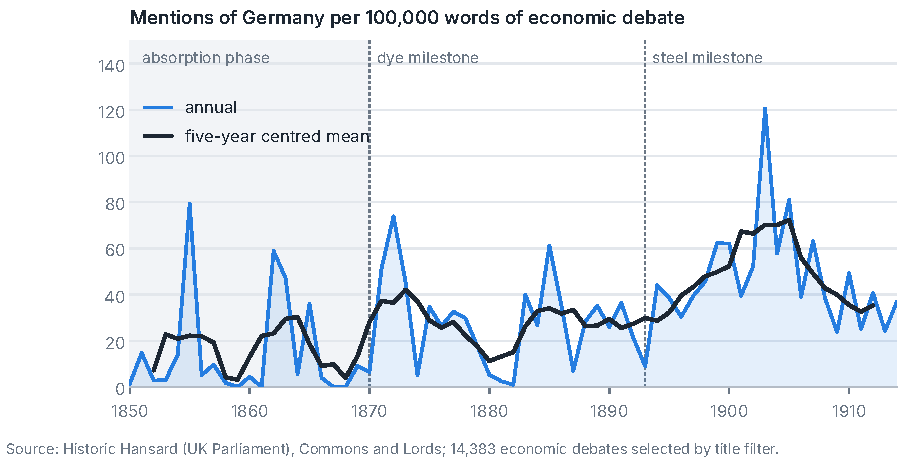
\includegraphics[width=0.9\textwidth,height=0.62\textheight,keepaspectratio]{figures/fig_e1_hansard.pdf}
\caption*{Figure E.1. Mentions of Germany per 100,000 words of British
economic debate, 1850-1914 (annual and five-year moving average).}
\end{figure}

Parliamentary attention to Germany roughly triples after the steel
milestone of 1893 and stays high through the Tariff Reform campaign.
Before 1870, Germany appears in economic debates mostly as a trading
partner or transit route, rather than as a competitor. The debates on
trade with Russia during the Crimean War are an example. A
structural-break search dates the shifts without imposing break dates in
advance. It uses log(1 + mentions per 100,000 words). The single best
break falls in 1871. When two breaks are allowed, they fall in 1871 and
1894, one year after the dye and the steel milestones. The Bayesian
information criterion (BIC), which trades fit against the number of
breaks, prefers one break over none by a wide margin
(\texttt{data/\allowbreak{}tests\_\allowbreak{}sequence.py}).

Two qualifications apply. First, the rise after 1871 is modest in level,
and the large increase comes after 1894. Second, the competition
indicator differs little between the 1850s and 1860s and the 1870s and
1880s. Its early annual values also rest on very few debates. The record
therefore appears to support the ordering, with attention following
displacement. It dates the escalation, however, to the second and
broader milestone.

\hypertarget{e.2-sector-debates}{%
\subsection*{E.2 Sector debates}\label{e.2-sector-debates}}

Aggregate attention mixes sectors with very different political weight.
A debate belongs to a sector if it uses at least three sector terms. It
links Germany to that sector if Germany appears within 30 words of a
sector term. We use the number of debates on a sector over the whole
period as a measure of its political voice. Census employment by sector
is not yet available as a check (Section K).

{\footnotesize\begin{longtable}[]{@{}
  >{\RaggedRight\arraybackslash}p{(\columnwidth - 8\tabcolsep) * \real{0.1593}}
  >{\RaggedRight\arraybackslash}p{(\columnwidth - 8\tabcolsep) * \real{0.1327}}
  >{\RaggedRight\arraybackslash}p{(\columnwidth - 8\tabcolsep) * \real{0.2832}}
  >{\RaggedRight\arraybackslash}p{(\columnwidth - 8\tabcolsep) * \real{0.2035}}
  >{\RaggedRight\arraybackslash}p{(\columnwidth - 8\tabcolsep) * \real{0.2212}}@{}}
\caption*{\textbf{Table E.2. Germany in British sector debates before and after
the sector milestone}}\\
\toprule\noalign{}
\begin{minipage}[b]{\linewidth}\raggedright
Sector
\end{minipage} & \begin{minipage}[b]{\linewidth}\raggedright
Milestone
\end{minipage} & \begin{minipage}[b]{\linewidth}\raggedright
Debates on the sector, 1850-1914
\end{minipage} & \begin{minipage}[b]{\linewidth}\raggedright
Germany linked, before
\end{minipage} & \begin{minipage}[b]{\linewidth}\raggedright
Germany linked, after
\end{minipage} \\
\midrule\noalign{}
\endhead
\bottomrule\noalign{}
\endlastfoot
Beet sugar & 1886 & 574 & 7.1 \% of 98 {[}3.5-14.0{]} & 17.0 \% of 476
{[}13.9-20.7{]} \\
Iron and steel & 1893 & 172 & 14.6 \% of 48 {[}7.2-27.2{]} & 24.2 \% of
124 {[}17.5-32.4{]} \\
Dyes and chemicals & 1870 & 18 & 0 of 1 & 29.4 \% of 17
{[}13.3-53.1{]} \\
\end{longtable}}

Brackets: 95 \% Wilson intervals.

The sharpest break occurs in sugar, the sector with the most political
voice. Germany is almost absent from British sugar debates before 1880
(2 of 75). It appears in 5 of 23 sugar debates in 1880-1885, before beet
imports overtook cane. From 1886 it appears in about one sugar debate in
six, and this run ends with the Brussels Sugar Convention of 1902. Steel
moves in the same direction, but its intervals overlap. Dyes, the sector
in which German displacement came first, were almost never debated. The
long lag between the dye milestone and the Patents and Designs Act of
1907 is consistent with this reading.

\hypertarget{e.3-export-data-by-sector}{%
\subsection*{E.3 Export data by sector}\label{e.3-export-data-by-sector}}

Tyszynski (1951, Tables G and II) reports manufactured exports of eleven
countries in sixteen groups for 1899 and 1913 (Table E.3). In chemicals,
German exports already exceeded British exports by 43 per cent in 1899.
This would be consistent with an early dye milestone. In iron and steel,
German exports were only 35 per cent of British exports in 1899 and
reached 91 per cent by 1913. In industrial equipment and electrical
goods, Germany overtook Britain between the two benchmark years.

The production crossover in steel (1893) thus preceded displacement in
export markets. That displacement came in the 1900s, when German
competition became a parliamentary theme and Tariff Reform was launched
(1903). Crafts (1989, Table 1) confirms the pattern from the side of
specialisation, using ranks of revealed comparative advantage. Chemicals
ranked among Germany's top five sectors in both 1899 and 1913. Iron and
steel did not (ranks 11 and 8). Electrical goods rose from rank 10 to
rank 1.

{\footnotesize\begin{longtable}[]{@{}
  >{\RaggedRight\arraybackslash}p{(\columnwidth - 8\tabcolsep) * \real{0.2439}}
  >{\RaggedRight\arraybackslash}p{(\columnwidth - 8\tabcolsep) * \real{0.1585}}
  >{\RaggedRight\arraybackslash}p{(\columnwidth - 8\tabcolsep) * \real{0.1585}}
  >{\RaggedRight\arraybackslash}p{(\columnwidth - 8\tabcolsep) * \real{0.2195}}
  >{\RaggedRight\arraybackslash}p{(\columnwidth - 8\tabcolsep) * \real{0.2195}}@{}}
\caption*{\textbf{Table E.3. German and American manufactured exports relative to
British exports, by group (Britain = 1)}}\\
\toprule\noalign{}
\begin{minipage}[b]{\linewidth}\raggedright
Group
\end{minipage} & \begin{minipage}[b]{\linewidth}\raggedright
Germany 1899
\end{minipage} & \begin{minipage}[b]{\linewidth}\raggedright
Germany 1913
\end{minipage} & \begin{minipage}[b]{\linewidth}\raggedright
United States 1899
\end{minipage} & \begin{minipage}[b]{\linewidth}\raggedright
United States 1913
\end{minipage} \\
\midrule\noalign{}
\endhead
\bottomrule\noalign{}
\endlastfoot
Iron and steel & 0.35 & 0.91 & 0.27 & 0.39 \\
Chemicals & 1.43 & 1.70 & 0.52 & 0.44 \\
Industrial equipment & 0.50 & 1.33 & 0.59 & 0.75 \\
Electrical goods & 0.58 & 2.11 & 0.94 & 0.69 \\
All manufactures & 0.68 & 0.89 & 0.34 & 0.42 \\
\end{longtable}}

Source: Tyszynski (1951), Tables G and II, current £000. We transcribed
the values from the scanned tables and checked them against the text
layer and the country totals in Table VIII. \# F. The United States as a
placebo before 1914

British attention to the United States did not rise when the United
States overtook Britain in income, which makes it a placebo case. The
United States overtook Britain in GDP per capita around 1900. The lead
changed hands several times in the 1890s and stayed with the United
States from 1899 (Bolt and van Zanden 2024). If growth alone triggered
escalation, British attention to the United States should have risen as
well. The debates show no such rise. Mentions of the United States per
100,000 words of economic debate stay between 41 and 56 across all four
periods of Table E.1. Mentions of Germany rise from 14 to 43-45. The
share of debates linking the United States to competition terms stays
between 0.7 and 2.1 per cent. It is highest in 1850-1869 and never above
the German share after 1893.

A phrase search finds no parliamentary echo of the press theme of an
`American invasion' around 1901. The phrase does not occur once in the
14,383 economic debates of 1850-1914. The phrase `American competition'
occurs in six debates in all, against eleven for `Made in Germany'
(\texttt{data/\allowbreak{}hansard\_\allowbreak{}phrases.py}).

Bilateral trade data suggest why. We use a fixed panel of 17 third
markets, that is, markets outside the three supplying countries. Each
has data for all three suppliers in every benchmark year from 1880 to
1913 (CEPII TRADHIST v4; Fouquin and Hugot 2016). In this panel, German
exports rise from 47 to 85 per cent of British exports. By 1913 they
exceed British exports in seven markets (Austria-Hungary, Belgium,
Denmark, Finland, Italy, Norway, Sweden). US exports rise from 46 to 75
per cent, but only to 51 per cent once Canada is excluded. They exceed
British exports only in Canada and Austria-Hungary (Table F.1).

{\footnotesize\begin{longtable}[]{@{}llll@{}}
\caption*{\textbf{Table F.1. Exports to 17 third markets relative to British
exports (Britain = 1)}}\\
\toprule\noalign{}
Year & United States & United States, without Canada & Germany \\
\midrule\noalign{}
\endhead
\bottomrule\noalign{}
\endlastfoot
1880 & 0.46 & 0.44 & 0.47 \\
1890 & 0.30 & 0.25 & 0.50 \\
1900 & 0.56 & 0.46 & 0.70 \\
1913 & 0.75 & 0.51 & 0.85 \\
\end{longtable}}

Markets: Argentina, Austria-Hungary, Belgium, Canada, Chile, Denmark,
Finland, France, British India, Italy, Japan, Norway, Ottoman Empire,
Portugal, Spain, Sweden, Uruguay. Flows are total goods in current
pounds and do not separate manufactures from primary goods.

Shares of world manufactured exports point the same way for manufactures
alone, in Tyszynski's (1951, Table VIII) figures. Between 1899 and 1913
the British share fell from 32.5 to 29.9 per cent. The German share rose
from 22.2 to 26.4 per cent. The American share rose only from 11.2 to
12.6 per cent. Relative to Britain, Germany moved from 0.68 to 0.88
(0.89 in Tables G and II, Table E.3), and the United States from 0.34 to
0.42. These figures suggest that the United States outgrew Britain at
home, while Germany displaced Britain in its export markets. \# G.
Congressional attention, 1955-2025

This section repeats the Hansard measure of Section E for the American
incumbent. The source is the Congressional Record, retrieved from the
govinfo API of the US Government Publishing Office. Code:
\texttt{data/\allowbreak{}crec\_\allowbreak{}fetch.py}, \texttt{data/\allowbreak{}crec\_\allowbreak{}filter.py},
\texttt{data/\allowbreak{}crec\_\allowbreak{}salience.py}, \texttt{data/\allowbreak{}crec\_\allowbreak{}sectors.py} (China);
\texttt{data/\allowbreak{}crecb\_\allowbreak{}fetch.py}, \texttt{data/\allowbreak{}crecb\_\allowbreak{}salience.py},
\texttt{data/\allowbreak{}crecb\_\allowbreak{}korea.py}, \texttt{data/\allowbreak{}crecb\_\allowbreak{}share.py},
\texttt{data/\allowbreak{}crecb\_\allowbreak{}controls.py} (Japan and Korea);
\texttt{data/\allowbreak{}crec\_\allowbreak{}controls.py} (China, controls);
\texttt{data/\allowbreak{}fr301\_\allowbreak{}lists.py} (Section 301 lists); break tests in
\texttt{data/\allowbreak{}tests\_\allowbreak{}sequence.py}.

\hypertarget{g.1-china-the-daily-record-1995-2025}{%
\subsection*{G.1 China: the daily Record,
1995-2025}\label{g.1-china-the-daily-record-1995-2025}}

\textbf{Data and filter.} The daily Congressional Record (collection
CREC) is divided into granules. A granule is one speech, debate or
insertion, and each has its own title. We exclude the Daily Digest and
front matter, which leaves 829,186 granules from 1995 to 2025. Of these,
10,901 carry an economic title under a fixed filter (version
\texttt{crec\_\allowbreak{}econ\_\allowbreak{}v1}). The filter terms are trade, tariff, import,
export, duties, customs, manufacturing, industry, dumping, subsidy,
competitiveness, currency, outsourcing, WTO, NAFTA, normal trade
relations, supply chain, intellectual property and the sector terms of
Table G.2. China counts when \emph{China}, \emph{Chinese}, \emph{PRC} or
\emph{Beijing} occurs. We first remove \emph{Republic of China}
(Taiwan). The competition indicator uses the Hansard list plus
\emph{manipulation}, \emph{overcapacity}, \emph{outsourcing},
\emph{offshoring} and \emph{counterfeit}.

{\footnotesize\begin{longtable}[]{@{}
  >{\RaggedRight\arraybackslash}p{(\columnwidth - 8\tabcolsep) * \real{0.1351}}
  >{\RaggedRight\arraybackslash}p{(\columnwidth - 8\tabcolsep) * \real{0.1532}}
  >{\RaggedRight\arraybackslash}p{(\columnwidth - 8\tabcolsep) * \real{0.1622}}
  >{\RaggedRight\arraybackslash}p{(\columnwidth - 8\tabcolsep) * \real{0.2613}}
  >{\RaggedRight\arraybackslash}p{(\columnwidth - 8\tabcolsep) * \real{0.2883}}@{}}
\caption*{\textbf{Table G.1. China in economic debates of the US Congress, pooled
by period}}\\
\toprule\noalign{}
\begin{minipage}[b]{\linewidth}\raggedright
Period
\end{minipage} & \begin{minipage}[b]{\linewidth}\raggedright
Economic granules
\end{minipage} & \begin{minipage}[b]{\linewidth}\raggedright
Mentioning China
\end{minipage} & \begin{minipage}[b]{\linewidth}\raggedright
China near a competition term
\end{minipage} & \begin{minipage}[b]{\linewidth}\raggedright
Mentions per 100,000 words: China / Japan / Mexico
\end{minipage} \\
\midrule\noalign{}
\endhead
\bottomrule\noalign{}
\endlastfoot
1995-2000 & 2,837 & 20.1 \% {[}18.6-21.6{]} & 5.2 \% {[}4.4-6.1{]} & 130
/ 34 / 35 \\
2001-2009 & 3,616 & 16.4 \% {[}15.2-17.6{]} & 6.8 \% {[}6.1-7.7{]} & 77
/ 16 / 27 \\
2010-2017 & 2,600 & 13.8 \% {[}12.5-15.2{]} & 6.6 \% {[}5.7-7.6{]} & 80
/ 9 / 21 \\
2018-2025 & 1,848 & 17.9 \% {[}16.2-19.7{]} & 7.5 \% {[}6.4-8.8{]} & 113
/ 6 / 35 \\
\end{longtable}}

Brackets: 95 \% Wilson intervals (confidence intervals for a
proportion).

\begin{figure}[htbp]
\centering
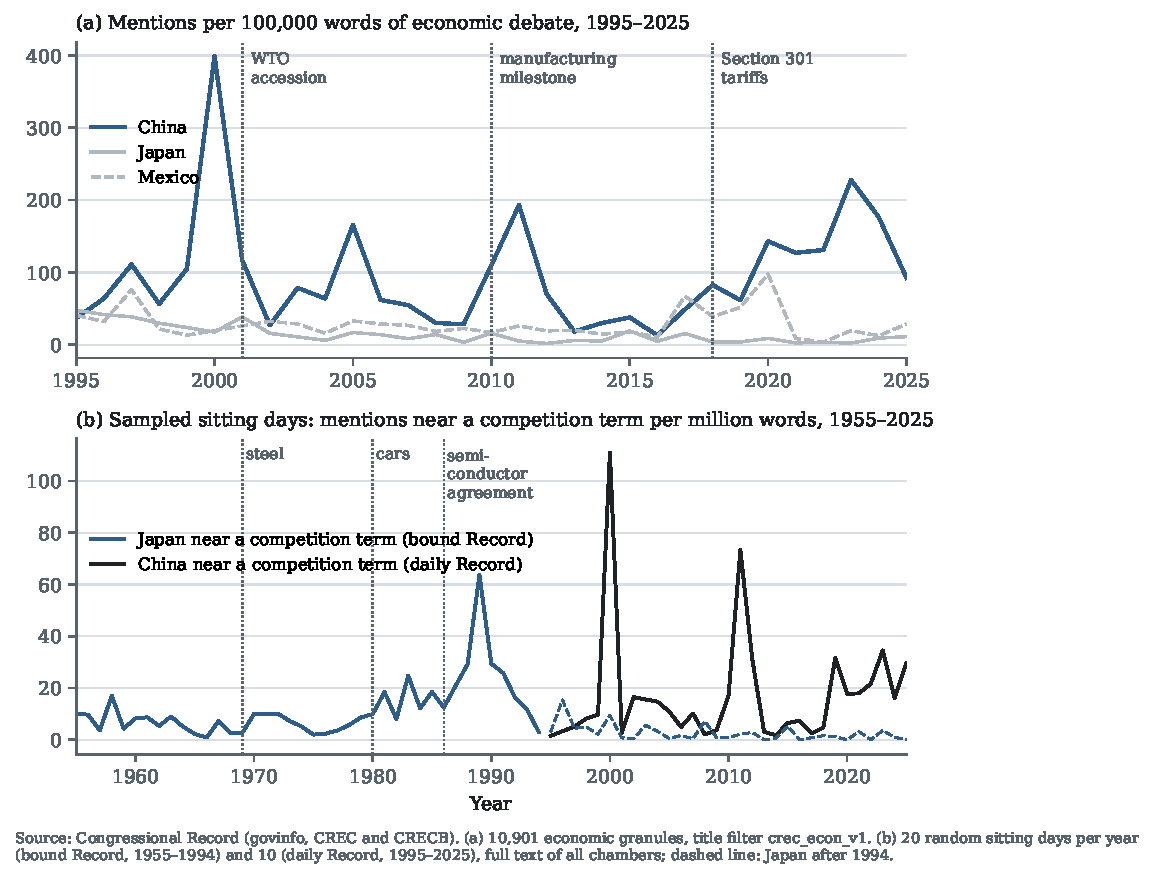
\includegraphics[width=0.9\textwidth,height=0.62\textheight,keepaspectratio]{figures/fig_e2_crec.pdf}
\caption*{Figure G.1. (a) China, Japan and Mexico in economic debates of
the US Congress, 1995-2025; (b) Japan and China near a competition term
on sampled sitting days, 1955-2025.}
\end{figure}

China was a subject in Congress before it displaced any American sector,
unlike Germany in the British record. Its trade status was itself the
subject of legislation. Congress renewed most-favoured-nation treatment
each year in the 1990s and granted permanent normal trade relations in
2000. That year marks the peak of the series, at 399 mentions per
100,000 words. Attention then falls back, with peaks in the currency
debates of 2005 and 2011, and rises again after 2018. The competition
indicator rises only slowly, from 5.2 to 7.5 per cent of economic
granules. We search for structural breaks and choose their number by the
Bayesian information criterion (BIC). On log(1 + mentions per 100,000
words) the BIC prefers no break. On the share of economic granules that
mention China, it places two breaks, in 2013 and 2018. These breaks mark
a trough before the tariffs of 2018. They do not mark a rise after the
export crossovers. The median crossover falls in 2004 under SITC
Revision 3 (70 groups) and in 2015 under the HS (242 groups).

\textbf{Coverage of the title filter.} A check sample measures what the
filter misses. It holds ten random sitting days per year (310 days,
46,357 granules), all retrieved in full. In 259 granules China appears
within 30 words of a competition term. Only 48 of these (19 per cent)
carry an economic title. The others are bill introductions,
appropriations and defence authorisations, nominations and amendment
texts. The sample-day measure in G.2 therefore uses the full text of the
sampled days.

{\footnotesize\begin{longtable}[]{@{}
  >{\RaggedRight\arraybackslash}p{(\columnwidth - 14\tabcolsep) * \real{0.1149}}
  >{\RaggedRight\arraybackslash}p{(\columnwidth - 14\tabcolsep) * \real{0.0862}}
  >{\RaggedRight\arraybackslash}p{(\columnwidth - 14\tabcolsep) * \real{0.1552}}
  >{\RaggedRight\arraybackslash}p{(\columnwidth - 14\tabcolsep) * \real{0.1724}}
  >{\RaggedRight\arraybackslash}p{(\columnwidth - 14\tabcolsep) * \real{0.1609}}
  >{\RaggedRight\arraybackslash}p{(\columnwidth - 14\tabcolsep) * \real{0.0862}}
  >{\RaggedRight\arraybackslash}p{(\columnwidth - 14\tabcolsep) * \real{0.1264}}
  >{\RaggedRight\arraybackslash}p{(\columnwidth - 14\tabcolsep) * \real{0.0977}}@{}}
\caption*{\textbf{Table G.2. China in congressional sector debates and broad
American instruments, by sector}}\\
\toprule\noalign{}
\begin{minipage}[b]{\linewidth}\raggedright
Sector
\end{minipage} & \begin{minipage}[b]{\linewidth}\raggedright
Crossover
\end{minipage} & \begin{minipage}[b]{\linewidth}\raggedright
Broad instrument (register)
\end{minipage} & \begin{minipage}[b]{\linewidth}\raggedright
China linked, before crossover
\end{minipage} & \begin{minipage}[b]{\linewidth}\raggedright
China linked, from crossover
\end{minipage} & \begin{minipage}[b]{\linewidth}\raggedright
Voice 2001-2017
\end{minipage} & \begin{minipage}[b]{\linewidth}\raggedright
Share on 301 lists 1-2
\end{minipage} & \begin{minipage}[b]{\linewidth}\raggedright
301 increase 2024
\end{minipage} \\
\midrule\noalign{}
\endhead
\bottomrule\noalign{}
\endlastfoot
Steel & ≤1992 & B-17, B-19 & n.a. & 17.4 \% of 430 & 8.04 & 0.00 &
yes \\
Aluminium & 2004 & B-19 & 11.1 \% of 9 & 20.6 \% of 34 & 0.32 & 0.03 &
yes \\
Solar cells & ≤2008 & B-18 & 0.0 \% of 19 & 25.9 \% of 108 & 2.41 & 1.00
& yes \\
Washing machines & 1999 & B-18 & 0.0 \% of 1 & 0.0 \% of 4 & 0.00 & 0.00
& no \\
Telecom equipment & 2003 & B-21 & 5.4 \% of 240 & 27.5 \% of 160 & 1.61
& 0.00 & no \\
Semiconductors & 2009 & B-22 & 16.7 \% of 60 & 42.2 \% of 64 & 1.29 &
1.00 & yes \\
Cars & 2023 & B-23 & 20.6 \% of 490 & 40.0 \% of 40 & 11.26 & 0.87 &
yes \\
Furniture & 2001 & n.a. & 0.0 \% of 17 & 34.1 \% of 41 & 2.09 & 0.00 &
no \\
Textiles and apparel & ≤1992 & n.a. & n.a. & 21.1 \% of 294 & 7.72 &
0.00 & yes \\
Footwear & ≤1992 & n.a. & n.a. & 21.5 \% of 93 & 2.25 & 0.00 & no \\
Toys & ≤1992 & n.a. & n.a. & 19.1 \% of 89 & 2.25 & 0.00 & no \\
Tyres & 2005 & n.a. & 12.0 \% of 25 & 32.0 \% of 25 & 1.29 & 0.07 &
no \\
Paper & ≤2008 & n.a. & 33.3 \% of 3 & 20.0 \% of 5 & 0.32 & 0.00 & no \\
Chemicals & 2004 & n.a. & 12.6 \% of 190 & 4.9 \% of 144 & 1.93 & 0.01 &
yes \\
Computers & 2003 & n.a. & 11.4 \% of 229 & 11.8 \% of 153 & 4.50 & 0.20
& no \\
Glass and ceramics & ≤1992 & n.a. & n.a. & 4.6 \% of 87 & 0.64 & 0.00 &
no \\
Batteries & 2004 & n.a. & 0.0 \% of 15 & 32.4 \% of 71 & 0.80 & 0.39 &
yes \\
\end{longtable}}

Sector debate: economic granule with at least three sector terms. China
linked: China within 30 words of a sector term. Crossover: earliest year
in which Chinese world exports of a group in the sector reached American
exports (\texttt{data/\allowbreak{}population\_\allowbreak{}crossovers.csv}; ≤ marks a crossover
in the first data year). Voice: China-linked sector debates per 1,000
economic granules, 2001-2017. Share on lists 1-2: mean share of the
sector's HTS8 lines (eight-digit tariff lines of the US tariff schedule)
on Section 301 lists 1 and 2, which carried 25 per cent from July and
August 2018. Instruments come from \texttt{data/\allowbreak{}broad\_\allowbreak{}register.csv},
without the economy-wide Section 301 tariffs (B-20). The 2024 increases
for textiles and chemicals concern face masks and critical minerals.

\textbf{Tests, China.} (a) \emph{Timing.} The timing comparison does not
separate displacement from trend. We use the nine sectors with an
uncensored crossover after 1999. China is linked to 14.0 per cent of
1,275 sector debates before the crossover {[}12.2-16.0{]} and to 22.4
per cent of 732 debates from the crossover {[}19.5-25.6{]}. Voice is
higher after the crossover in four of nine sectors. Attention to China
in all debates also rises over time, however, so the rise need not
reflect displacement.

\begin{enumerate}
\def\labelenumi{(\alph{enumi})}
\setcounter{enumi}{1}
\item
  \emph{Selection.} Sectors that later received a sector-specific broad
  measure had more China-linked debates than displaced sectors without
  one, but none of the differences is significant. We use exact
  one-sided permutation tests. Voice in 2001-2017 is 3.6 against 2.4 (p
  = 0.25). In the five years before the crossover p = 0.43. In the five
  years from the crossover voice is 4.8 against 1.4 (p = 0.17). The
  number of economic debates on a sector does not separate the groups
  significantly either (237 against 148 debates, p = 0.15). Nor does the
  share of debates linking China (25 against 20 per cent from the
  crossover, p = 0.22). Import volume and employment do not separate the
  two groups (p = 0.36 and 0.32). The register leaves out the Section
  421 tyre safeguard of 2009 and the textile safeguards of 2005, because
  they fall outside its Section 201 rule. Counting them as broad
  measures changes little (p = 0.11 for voice 2001-2017).
\item
  \emph{Graded tariffs.} The Section 301 tariffs of 2018 covered all
  groups, but not equally. Lists 1 and 2 took effect first, at 25 per
  cent. They concentrated on machinery, electronics, vehicles and
  plastics, the targets of Made in China 2025. Congressional voice does
  not predict a sector's share on lists 1 and 2. The rank correlation
  (Spearman ρ) is 0.06 across 17 sectors. Among 229 displaced HS4 groups
  (four-digit HS headings), an ordinary least squares (OLS) regression
  gives a coefficient of 0.06 (p = 0.50). It holds import volume and
  employment constant and clusters standard errors in 13 sector groups.
  Voice is weakly associated with the sector increases of the 2024
  review (voice 4.2 against 1.7, p = 0.056).
\end{enumerate}

\textbf{Controls, China.} None of the three size measures predicts a
sector-specific broad measure against China in the expected direction.
The data cover the 17 Chinese sectors
(\texttt{data/\allowbreak{}ds1\_\allowbreak{}crec\_\allowbreak{}controls.txt}). Volume is the number of
economic debates on the sector per 1,000 economic granules in 2001-2017.
Employment and imports are computed for every Chinese crossover group in
its crossover year. They are summed within the classification that dates
the sector's crossover. The values match
\texttt{data/\allowbreak{}population\_\allowbreak{}weight.csv} exactly for the 116 groups in both
files. Taken alone, volume has a coefficient of 0.04 per log point
(permutation p = 0.39), employment −0.19 (p = 0.87 for a positive
effect) and imports −0.21. With all three together, volume is positive
but not significant (0.13, p = 0.16). Imports are negative (−0.24, p =
0.025 with HC1 robust standard errors). The sectors that drew measures
against China had lower American imports from China at the crossover
than consumer-goods sectors that drew none, such as computers,
furniture, toys and footwear. At the level of 330 groups, employment is
positive once volume and imports are held constant (0.61, p = 0.010).
This result rests on many groups in few sectors (17 clusters), and it
does not appear at the sector level.

\textbf{Section 301 lists.} The lists come from the Federal Register:
list 1, 83 FR 28710 (Annex A, 817 lines read); list 2, 83 FR 40823
(283); list 3, 83 FR 47974 (5,748); lists 4A and 4B, 84 FR 43304 (3,233
and 550); four-year review, 89 FR 76581 (Annex A, 387 of 389 lines). In
the review we identify 11 of 14 product groups, because three share
lines with others. Our counts differ by a few lines from USTR's totals,
because some codes also occur in the notes.

\hypertarget{g.2-japan-and-korea-the-bound-record-1955-1994}{%
\subsection*{G.2 Japan and Korea: the bound Record,
1955-1994}\label{g.2-japan-and-korea-the-bound-record-1955-1994}}

\textbf{Data.} Before 1995 the Record exists in machine-readable form
only as the bound edition (collection CRECB). It holds one PDF with a
text layer per sitting day and chamber, and it has no debate titles. We
draw 20 random sitting days per year from 1955 to 1994, with the seed
fixed in the code. This gives 800 days, covering the House, the Senate
and the Extensions of Remarks. We read the full text with pdftotext.
Without titles no economic filter is possible. The measure therefore
counts the places where the challenger stands within 30 words of a
competition term or a sector term, per million words of the whole day.
For comparison over time, we compute the same measure on the 310 check
days of the daily Record (1995-2025). In all, this gives 1,110 days and
279 million words. For Korea, we first remove mentions that do not refer
to the South Korean economy (\emph{North Korea(n)}, \emph{Democratic
People's Republic of Korea}, \emph{Korean War}, \emph{Korean conflict},
\emph{Korean peninsula}). Korea counts at \emph{Korea},
\emph{Korean(s)}, \emph{Korea's} and \emph{Seoul}.

{\footnotesize\begin{longtable}[]{@{}
  >{\RaggedRight\arraybackslash}p{(\columnwidth - 6\tabcolsep) * \real{0.1351}}
  >{\RaggedRight\arraybackslash}p{(\columnwidth - 6\tabcolsep) * \real{0.2883}}
  >{\RaggedRight\arraybackslash}p{(\columnwidth - 6\tabcolsep) * \real{0.2883}}
  >{\RaggedRight\arraybackslash}p{(\columnwidth - 6\tabcolsep) * \real{0.2883}}@{}}
\caption*{\textbf{Table G.3. Japan and China near a competition term on sampled
sitting days of Congress}}\\
\toprule\noalign{}
\begin{minipage}[b]{\linewidth}\raggedright
Period
\end{minipage} & \begin{minipage}[b]{\linewidth}\raggedright
Japan, mentions per 100,000 words
\end{minipage} & \begin{minipage}[b]{\linewidth}\raggedright
Japan near a competition term, per million words
\end{minipage} & \begin{minipage}[b]{\linewidth}\raggedright
China near a competition term, per million words
\end{minipage} \\
\midrule\noalign{}
\endhead
\bottomrule\noalign{}
\endlastfoot
1955-1964 & 11.2 & 8.2 & 2.6 \\
1965-1974 & 12.1 & 6.1 & 1.8 \\
1975-1984 & 13.1 & 8.9 & 2.4 \\
1985-1994 & 21.0 & 21.9 & 3.4 \\
1995-2004 & 6.3 & 4.9 & 19.9 \\
2005-2014 & 4.3 & 1.4 & 14.8 \\
2015-2025 & 5.4 & 1.8 & 16.5 \\
\end{longtable}}

Attention to Japan as a competitor stays low and steady through the
1960s and 1970s and rises in the 1980s. In the earlier decades Japanese
textiles, steel and television sets overtook American exports. A break
search on log(1 + Japan near a competition term) places the best single
break in 1980, the year of the car milestone (BIC −33.8 against −23.3
without a break). With two breaks, it places them in 1964 and 1980. The
sample-day series for China prefers no break. On this common measure,
congressional attention to China as a competitor after 1995 was of the
same order as attention to Japan in the late 1980s. It was already high
in the first years of the series, before most Chinese crossovers. Korea
near a competition term rises from 0.7 per million words in 1955-1964 to
1.2 in 1975-1984 and 2.6 in 1985-1994. This is about a tenth of the
level for Japan. It peaks at 6.8 in 2005-2014, the years of the
bilateral free trade agreement. A break search prefers no break.

\textbf{Raw sector counts.} Tables G.4 and G.5 report, by sector, how
often Congress mentioned the challenger near a sector term. These counts
mix two things: how much Congress talks about a sector, and how much of
that talk names the challenger. We therefore report tests only on the
size-adjusted measures of Table G.6.

{\footnotesize\begin{longtable}[]{@{}
  >{\RaggedRight\arraybackslash}p{(\columnwidth - 10\tabcolsep) * \real{0.1408}}
  >{\RaggedRight\arraybackslash}p{(\columnwidth - 10\tabcolsep) * \real{0.1620}}
  >{\RaggedRight\arraybackslash}p{(\columnwidth - 10\tabcolsep) * \real{0.2254}}
  >{\RaggedRight\arraybackslash}p{(\columnwidth - 10\tabcolsep) * \real{0.1901}}
  >{\RaggedRight\arraybackslash}p{(\columnwidth - 10\tabcolsep) * \real{0.1761}}
  >{\RaggedRight\arraybackslash}p{(\columnwidth - 10\tabcolsep) * \real{0.1056}}@{}}
\caption*{\textbf{Table G.4. Japan near sector terms on sampled days, per million
words}}\\
\toprule\noalign{}
\begin{minipage}[b]{\linewidth}\raggedright
Sector
\end{minipage} & \begin{minipage}[b]{\linewidth}\raggedright
Crossover (SITC Rev.~1)
\end{minipage} & \begin{minipage}[b]{\linewidth}\raggedright
Broad instrument (register)
\end{minipage} & \begin{minipage}[b]{\linewidth}\raggedright
Five years before crossover
\end{minipage} & \begin{minipage}[b]{\linewidth}\raggedright
Five years from crossover
\end{minipage} & \begin{minipage}[b]{\linewidth}\raggedright
1960-1975
\end{minipage} \\
\midrule\noalign{}
\endhead
\bottomrule\noalign{}
\endlastfoot
Textiles and apparel & ≤1962 & B-01, B-02, B-04 (from 1957) & 13.65 &
1.95 & 4.39 \\
Steel & ≤1962 & B-03, B-05, B-09, B-12, B-13, B-17 (from 1969) & 2.20 &
3.66 & 2.80 \\
Television sets & 1965 & B-07, B-16 (from 1977) & 0.63 & 0.41 & 0.88 \\
Cars and motorcycles & 1977 & B-10, B-11 (from 1981) & 1.16 & 5.69 &
1.26 \\
Semiconductors & 1989 & B-14, B-16 (from 1986) & 5.55 & 3.85 & 0.06 \\
Machine tools & 1977 & B-15 (from 1986) & 0.17 & 0.32 & 0.11 \\
Ships & ≤1962 & n.a. & 0.47 & 0.24 & 0.48 \\
Footwear & ≤1962 & n.a. & 0.21 & 0.62 & 0.71 \\
Cameras and optics & 1977 & n.a. & 0.03 & 0.25 & 0.20 \\
Toys & ≤1962 & n.a. & 0.21 & 0.10 & 0.09 \\
Glass and ceramics & ≤1962 & n.a. & 0.63 & 0.43 & 0.55 \\
Ball bearings & 1986 & n.a. & 0.00 & 0.11 & 0.01 \\
Tyres & 1969 & n.a. & 0.16 & 0.12 & 0.13 \\
Plywood & ≤1962 & n.a. & 12.07 & 0.14 & 0.22 \\
\end{longtable}}

Crossover: earliest year in which Japanese world exports in a group of
the sector reached American exports (≤: in the first data year, 1962).
Instruments from \texttt{data/\allowbreak{}broad\_\allowbreak{}register.csv}.

{\footnotesize\begin{longtable}[]{@{}
  >{\RaggedRight\arraybackslash}p{(\columnwidth - 10\tabcolsep) * \real{0.1399}}
  >{\RaggedRight\arraybackslash}p{(\columnwidth - 10\tabcolsep) * \real{0.1958}}
  >{\RaggedRight\arraybackslash}p{(\columnwidth - 10\tabcolsep) * \real{0.1958}}
  >{\RaggedRight\arraybackslash}p{(\columnwidth - 10\tabcolsep) * \real{0.1888}}
  >{\RaggedRight\arraybackslash}p{(\columnwidth - 10\tabcolsep) * \real{0.1748}}
  >{\RaggedRight\arraybackslash}p{(\columnwidth - 10\tabcolsep) * \real{0.1049}}@{}}
\caption*{\textbf{Table G.5. Korea near sector terms on sampled days, per million
words}}\\
\toprule\noalign{}
\begin{minipage}[b]{\linewidth}\raggedright
Sector
\end{minipage} & \begin{minipage}[b]{\linewidth}\raggedright
Crossover (SITC Rev.~1 or 3)
\end{minipage} & \begin{minipage}[b]{\linewidth}\raggedright
Broad instrument (register)
\end{minipage} & \begin{minipage}[b]{\linewidth}\raggedright
Five years before crossover
\end{minipage} & \begin{minipage}[b]{\linewidth}\raggedright
Five years from crossover
\end{minipage} & \begin{minipage}[b]{\linewidth}\raggedright
1965-1990
\end{minipage} \\
\midrule\noalign{}
\endhead
\bottomrule\noalign{}
\endlastfoot
Textiles and apparel & 1970 & B-02, B-04 (from 1962) & 0.15 & 1.26 &
0.83 \\
Footwear & 1972 & B-06 (from 1977) & 0.00 & 0.17 & 0.23 \\
Television sets & ≤1992 & B-08 (from 1979) & 0.51 & 0.12 & 0.25 \\
Steel & 1977 & B-13, B-17, B-19 (from 1984) & 0.30 & 0.18 & 0.38 \\
Washing machines & 2002 & B-18 (from 2018) & 0.00 & 0.00 & 0.01 \\
Ships & 1977 & n.a. & 0.11 & 0.14 & 0.10 \\
Telecom equipment & 2003 & n.a. & 0.06 & 0.07 & 0.12 \\
Plywood & 1968 & n.a. & 0.00 & 0.00 & 0.00 \\
Leather & ≤1992 & n.a. & 0.00 & 0.00 & 0.05 \\
Travel goods & 1974 & n.a. & 0.00 & 0.06 & 0.01 \\
Glass and ceramics & 1979 & n.a. & 0.11 & 0.08 & 0.08 \\
Toys & 1985 & n.a. & 0.00 & 0.00 & 0.01 \\
Copper, zinc, nickel & 1988 & n.a. & 0.00 & 0.00 & 0.03 \\
Optical goods & 1991 & n.a. & 0.07 & 0.04 & 0.04 \\
\end{longtable}}

{\footnotesize\begin{longtable}[]{@{}
  >{\RaggedRight\arraybackslash}p{(\columnwidth - 12\tabcolsep) * \real{0.0941}}
  >{\RaggedRight\arraybackslash}p{(\columnwidth - 12\tabcolsep) * \real{0.1176}}
  >{\RaggedRight\arraybackslash}p{(\columnwidth - 12\tabcolsep) * \real{0.0941}}
  >{\RaggedRight\arraybackslash}p{(\columnwidth - 12\tabcolsep) * \real{0.1882}}
  >{\RaggedRight\arraybackslash}p{(\columnwidth - 12\tabcolsep) * \real{0.1882}}
  >{\RaggedRight\arraybackslash}p{(\columnwidth - 12\tabcolsep) * \real{0.1647}}
  >{\RaggedRight\arraybackslash}p{(\columnwidth - 12\tabcolsep) * \real{0.1529}}@{}}
\caption*{\textbf{Table G.6. Size-adjusted measures: sector volume and the
challenger's share of it (sampled days)}}\\
\toprule\noalign{}
\begin{minipage}[b]{\linewidth}\raggedright
Challenger
\end{minipage} & \begin{minipage}[b]{\linewidth}\raggedright
Sector
\end{minipage} & \begin{minipage}[b]{\linewidth}\raggedright
Broad instrument
\end{minipage} & \begin{minipage}[b]{\linewidth}\raggedright
Sector volume, five years before crossover
\end{minipage} & \begin{minipage}[b]{\linewidth}\raggedright
Sector volume, five years from crossover
\end{minipage} & \begin{minipage}[b]{\linewidth}\raggedright
Challenger share, before (\%)
\end{minipage} & \begin{minipage}[b]{\linewidth}\raggedright
Challenger share, from (\%)
\end{minipage} \\
\midrule\noalign{}
\endhead
\bottomrule\noalign{}
\endlastfoot
Japan & Textiles and apparel & yes & 309.9 & 203.9 & 5.5 & 1.2 \\
Japan & Steel & yes & 91.9 & 66.2 & 2.4 & 5.2 \\
Japan & Television sets & yes & 92.3 & 104.9 & 0.4 & 0.5 \\
Japan & Cars and motorcycles & yes & 131.0 & 88.8 & 0.9 & 5.6 \\
Japan & Semiconductors & yes & 34.1 & 18.0 & 17.2 & 18.9 \\
Japan & Machine tools & yes & 4.2 & 2.3 & 3.9 & 6.3 \\
Japan & Ships & no & 22.0 & 20.8 & 2.4 & 0.7 \\
Japan & Footwear & no & 10.2 & 18.3 & 2.0 & 3.1 \\
Japan & Cameras and optics & no & 11.0 & 8.0 & 0.2 & 3.1 \\
Japan & Toys & no & 2.3 & 1.9 & 7.0 & 5.1 \\
Japan & Glass and ceramics & no & 31.0 & 20.5 & 2.2 & 1.9 \\
Japan & Ball bearings & no & 1.1 & 1.0 & 0.0 & 7.4 \\
Japan & Tyres & no & 28.6 & 34.3 & 0.3 & 0.4 \\
Japan & Plywood & no & 33.4 & 5.1 & 43.4 & 0.9 \\
Korea & Textiles and apparel & yes & 132.0 & 121.9 & 0.1 & 1.5 \\
Korea & Footwear & yes & 22.4 & 17.5 & 0.0 & 0.8 \\
Korea & Television sets & yes & 99.8 & 135.9 & 0.4 & 0.1 \\
Korea & Steel & yes & 51.4 & 76.5 & 0.5 & 0.3 \\
Korea & Washing machines & yes & 6.0 & 7.5 & 0.0 & 0.0 \\
Korea & Ships & no & 11.4 & 18.7 & 0.7 & 1.0 \\
Korea & Telecom equipment & no & 62.0 & 34.2 & 0.1 & 0.4 \\
Korea & Plywood & no & 6.2 & 3.8 & 0.0 & 0.0 \\
Korea & Leather & no & 3.2 & 2.2 & 0.0 & 0.0 \\
Korea & Travel goods & no & 1.7 & 1.1 & 0.0 & 5.1 \\
Korea & Glass and ceramics & no & 18.9 & 13.3 & 0.6 & 0.6 \\
Korea & Toys & no & 4.3 & 7.3 & 0.0 & 0.0 \\
Korea & Copper, zinc, nickel & no & 12.8 & 9.0 & 0.0 & 0.0 \\
Korea & Optical goods & no & 11.2 & 14.6 & 0.6 & 0.3 \\
\end{longtable}}

Sector volume: mentions of the sector terms per million words of all
sampled days. Challenger share: per cent of those mentions with Japan
(Korea) within 30 words (\texttt{data/\allowbreak{}crecb\_\allowbreak{}share.py},
\texttt{data/\allowbreak{}ds1\_\allowbreak{}share\_\allowbreak{}test.txt}).

\textbf{Tests, Japan and Korea.} The challenger's share of sector talk
does not separate the sectors that drew a broad measure from those that
did not. For Japan the share from the crossover is 6.3 against 2.8 per
cent (exact one-sided permutation test, p = 0.11). Before the crossover
it is 5.0 against 7.2 per cent (p = 0.51). For Korea the share from the
crossover is 0.5 against 0.8 per cent (p = 0.48), and before it p =
0.59. Sector volume does separate the two groups, and already before
displacement. In the five years before the crossover, Congress mentioned
the Japanese sectors that later drew a broad measure 111 times per
million words, and the others 17 times (p = 0.006). For Korea the
figures are 62 against 15 (p = 0.020). From the crossover, p = 0.010 for
both. The selection of displaced sectors for broad measures therefore
appears to follow how much Congress debated a sector before
displacement. Attention to the particular challenger does not appear to
drive it. This matches the Hansard definition of voice (Section E.2).
The sector terms differ in breadth: \emph{television} also covers
broadcasting, and \emph{cars} also covers railway cars. This inflates
the volume of some large sectors. The ordering does not rest on these
terms alone, since textiles and steel lead in both cases.

\textbf{Controls, Japan and Korea.} Sector volume keeps its effect once
the size of the American industry is held constant. Volume is correlated
with that size (Spearman 0.38 with employment, 0.24 with imports from
the challenger). We therefore regress the indicator for a broad measure
on three variables: log sector volume before the crossover, log American
employment and log American imports from the challenger in the crossover
year. The model includes a country indicator
(\texttt{data/\allowbreak{}crecb\_\allowbreak{}controls.py},
\texttt{data/\allowbreak{}ds1\_\allowbreak{}share\_\allowbreak{}controls.txt}). We compute employment and
imports for every displaced group by the rules of Section D, including
groups that crossed in the first data year. Employment comes from the
NBER-CES manufacturing database, distributed to groups through the
Census concordance of 2002 and held at its 1958 level before 1958.
Imports come from UN Comtrade. For the 79 groups already in
\texttt{data/\allowbreak{}population\_\allowbreak{}weight.csv}, the values match exactly. All 28
sectors enter (Japan 14, Korea 14; 11 with a broad measure). Taken
alone, each variable predicts a broad measure: volume (coefficient 0.22
per log point, permutation p = 0.002), employment (0.18, p = 0.009) and
imports (0.11, p = 0.007). Taken together, volume keeps most of its
coefficient (0.18, permutation p = 0.011, 10,000 draws within country).
Employment loses its effect (p = 0.33). Imports keep a smaller,
borderline effect (0.08, p = 0.084). We repeat the test at the level of
the 63 displaced groups, with the sector's measure as outcome and
standard errors clustered by sector. The result is the same (volume p =
0.021, employment p = 0.75, imports p = 0.40). Congressional volume thus
appears to carry information that the size of the industry and its
exposure to imports do not.

\textbf{Limits of the congressional measures.} The congressional
measures have four limits. First, the sample of days is small for sector
counts in single years. Second, the text layer of the bound Record
contains OCR errors and runs adjacent columns together, which blurs the
30-word window. The noise does not appear to rise over time, however.
The share of 20 common English function words in all word tokens is
similar in 1958, 1970 and 1985 (0.32, 0.30 and 0.30). Each year uses
five sampled days, with 0.9 to 1.6 million words per year
(\texttt{data/\allowbreak{}crecb\_\allowbreak{}ocr\_\allowbreak{}check.py}). Third, the title filter of the
daily Record misses most economic discussion of China (G.1). Fourth, the
measures count attention, not lobbying or votes. \# H. Further cases

We apply the rules of Sections B to D to eight further dyads, that is,
pairs of challenger and incumbent. Code: \texttt{data/\allowbreak{}cases\_\allowbreak{}fetch.py},
\texttt{data/\allowbreak{}cases\_\allowbreak{}test.py} (output \texttt{data/\allowbreak{}cases\_\allowbreak{}panel.txt},
\texttt{data/\allowbreak{}cases\_\allowbreak{}breadth.csv}, \texttt{data/\allowbreak{}cases\_\allowbreak{}crossovers.csv},
\texttt{data/\allowbreak{}cases\_\allowbreak{}hazard.csv},
\texttt{data/\allowbreak{}cases\_\allowbreak{}register\_\allowbreak{}tested.csv}),
\texttt{data/\allowbreak{}third\_\allowbreak{}markets\_\allowbreak{}1930s.py}, \texttt{data/\allowbreak{}hansard\_\allowbreak{}japan.py},
\texttt{data/\allowbreak{}tests\_\allowbreak{}sequence.py}.

\hypertarget{h.1-data}{%
\subsection*{H.1 Data}\label{h.1-data}}

We use world exports by reporter from UN Comtrade in three
classifications. These are the Standard International Trade
Classification (SITC) Rev.~1 (1962-1999), SITC Rev.~3 (1992-2009) and
the Harmonized System (HS) at four digits (2008-2023). Taiwan reports
only in HS. For SITC, we take its exports as the imports of all
reporters from partner 490 (``Other Asia, nes''). We compare these with
the same reporters' imports from the United States, and both are valued
c.i.f., that is, including cost, insurance and freight. For Hong Kong we
use exports minus re-exports, and re-exports by product are available
only to 2016. For Japan against Britain we use CEPII TRADHIST v4. It
gives total bilateral exports to 35 markets with values for both
suppliers in every year 1924-1938, without Japan's colonies.

{\footnotesize\begin{longtable}[]{@{}
  >{\RaggedRight\arraybackslash}p{(\columnwidth - 6\tabcolsep) * \real{0.1684}}
  >{\RaggedRight\arraybackslash}p{(\columnwidth - 6\tabcolsep) * \real{0.1579}}
  >{\RaggedRight\arraybackslash}p{(\columnwidth - 6\tabcolsep) * \real{0.3368}}
  >{\RaggedRight\arraybackslash}p{(\columnwidth - 6\tabcolsep) * \real{0.3368}}@{}}
\caption*{\textbf{Table H.1. Reach of displacement: share of American manufactured
exports in groups the challenger had overtaken (challenger exports ≥ US
exports and ≥ USD 50 million)}}\\
\toprule\noalign{}
\begin{minipage}[b]{\linewidth}\raggedright
Challenger
\end{minipage} & \begin{minipage}[b]{\linewidth}\raggedright
Data
\end{minipage} & \begin{minipage}[b]{\linewidth}\raggedright
Selected years
\end{minipage} & \begin{minipage}[b]{\linewidth}\raggedright
Peak
\end{minipage} \\
\midrule\noalign{}
\endhead
\bottomrule\noalign{}
\endlastfoot
Japan & SITC 1 & 0.31 (1977), 0.27 (1981), 0.35 (1987) & 0.48 (1995) \\
China & HS & 0.45 (2018) & 0.55 (2023) \\
Korea & SITC 1 / 3 & 0.024 (1977), 0.027 (1984), 0.024 (2002) & 0.054
(1988, SITC 1); 0.074 (2009, SITC 3) \\
Taiwan & SITC 1 / 3 / HS & 0.011 (1977), 0.031 (1986), 0.087 (2023) &
0.045 (1987, SITC 1); 0.095 (2005, SITC 3) \\
Vietnam & HS & 0.048 (2018), 0.064 (2023) & 0.064 (2023) \\
Mexico & HS & 0.066 (2023) & 0.083 (2022) \\
Malaysia & HS & 0.045 (2023) & 0.060 (2021) \\
Hong Kong & SITC 1 & 0.020 (1988) & 0.022 (1987) \\
Thailand & HS & 0.014 (2023) & 0.016 (2022) \\
Brazil & SITC 1 / HS & 0.007 (1984), 0.008 (2023) & 0.011 (2013) \\
\end{longtable}}

\hypertarget{h.2-register-extension}{%
\subsection*{H.2 Register extension}\label{h.2-register-extension}}

The extension adds nineteen entries to the register (B-24 to B-42 in
\texttt{data/\allowbreak{}broad\_\allowbreak{}register.csv}). Each entry has its primary source:

\begin{itemize}
\tightlist
\item
  footwear orderly marketing agreement (OMA) with Taiwan, June 1977
  (Proclamation 4510);
\item
  colour-television OMA with Taiwan, 1979 (Proclamation 4634);
\item
  steel voluntary restraint agreements (VRAs) with Brazil and Mexico,
  1984 (Moore 1996, Table 2.8);
\item
  machine-tool VRA with Taiwan, 1986 (Dinopoulos and Kreinin 1991);
\item
  100 per cent tariffs on Brazilian goods, October 1988 (Proclamation
  5885);
\item
  graduation of Hong Kong and Taiwan from the US Generalised System of
  Preferences (GSP), effective 1989 (Proclamation 5805);
\item
  US-Vietnam textile agreement, May 2003 (FR Doc. 03-12314);
\item
  quotas under the Multifibre Arrangement (MFA) and the Agreement on
  Textiles and Clothing (ATC) on Taiwan, Hong Kong, Thailand, Malaysia,
  Brazil and Mexico, in force 1994-2004 by Federal Register notices;
\item
  end of Hong Kong's differential treatment, 2020 (executive order, EO
  13936);
\item
  tariffs under the International Emergency Economic Powers Act (IEEPA),
  2025, on Mexico (EO 14194), all partners (EO 14257, 14326), Brazil (EO
  14323) and Hong Kong (EO 14257).
\end{itemize}

The MFA and ATC quotas are excluded from the hazard analysis below. The
first agreements with these partners are already entered as B-37 to
B-42.

Six of the entries (B-37 to B-42) date the first comprehensive US cotton
textile agreement with each economy from Federal Register notices. The
dates are Hong Kong (35 categories, from 1 October 1963), Taiwan (19
October 1963), Mexico (2 June 1967), Brazil (23 October 1970), Malaysia
(1 September 1970; USITC Pub. 850, p.~50) and Thailand (16 March 1972).
Earlier restraints on single categories are recorded in the notes and
scored 3 on the reach score (IR). They cover Hong Kong from 3 March
1962, Taiwan from 23 June 1962, Mexico from 10 August 1962, Brazil from
October 1963 and Malaysia from August 1966. A restraint on Thailand was
requested in April 1971. The Multifibre Arrangement was concluded at
Geneva on 20 December 1973 and entered into force on 1 January 1974
(Article 14(1); text reproduced in USITC Pub. 850, Appendix A).

In the next table, the phase column compares each instrument with the
export crossover of the groups it covered. ``Post'' marks an instrument
after the crossover, and ``absorption'' one before it.

{\footnotesize\begin{longtable}[]{@{}
  >{\RaggedRight\arraybackslash}p{(\columnwidth - 8\tabcolsep) * \real{0.2222}}
  >{\RaggedRight\arraybackslash}p{(\columnwidth - 8\tabcolsep) * \real{0.2222}}
  >{\RaggedRight\arraybackslash}p{(\columnwidth - 8\tabcolsep) * \real{0.1111}}
  >{\RaggedRight\arraybackslash}p{(\columnwidth - 8\tabcolsep) * \real{0.2222}}
  >{\RaggedRight\arraybackslash}p{(\columnwidth - 8\tabcolsep) * \real{0.2222}}@{}}
\caption*{\textbf{Table H.2. Broad instruments against the further cases and the
crossover of the groups they covered}}\\
\toprule\noalign{}
\begin{minipage}[b]{\linewidth}\raggedright
Instrument
\end{minipage} & \begin{minipage}[b]{\linewidth}\raggedright
Target
\end{minipage} & \begin{minipage}[b]{\linewidth}\raggedright
IR
\end{minipage} & \begin{minipage}[b]{\linewidth}\raggedright
Crossover of covered groups
\end{minipage} & \begin{minipage}[b]{\linewidth}\raggedright
Phase
\end{minipage} \\
\midrule\noalign{}
\endhead
\bottomrule\noalign{}
\endlastfoot
Footwear OMA 1977 & Taiwan & 4 & 1970 & post \\
Colour-TV OMA 1979 & Taiwan & 4 & none & extension of instrument against
Japan \\
Steel VRAs 1984 & Brazil & 4 & 1983 & post \\
Steel VRAs 1984 & Mexico & 4 & none & extension \\
Machine-tool VRA 1986 & Taiwan & 4 & none & extension of instrument
against Japan \\
Section 301 tariffs 1988 & Brazil & 4 & none & retaliation over
patents \\
GSP graduation 1989 & Hong Kong, Taiwan & 4 (doubtful) & none
(economy-wide) & rule-based \\
Cotton textile agreements 1963 & Hong Kong; Taiwan & 4 & 1965; 1971 &
absorption (2 and 8 years) \\
Cotton textile agreements 1967-1972 & Mexico; Brazil; Malaysia; Thailand
& 4 & none & restraint without displacement \\
Textile agreement 2003 & Vietnam & 4 & 2006 (apparel, SITC 84, all
covered groups summed; groups 841 and 842 alone in 2002) & absorption (3
years) \\
End of differential treatment 2020 & Hong Kong & 5 & none & political \\
IEEPA tariffs 2025 & Mexico; Brazil; Hong Kong & 5 & none (economy-wide)
& political \\
Reciprocal tariffs 2025 & all partners & 5 & none (economy-wide) &
global, deficit-based \\
\end{longtable}}

\hypertarget{h.3-hazard-and-control-group}{%
\subsection*{H.3 Hazard and control
group}\label{h.3-hazard-and-control-group}}

Most displaced groups in the further cases drew no targeted sectoral
broad measure within ten years. We count the groups whose crossover does
not fall in the first data year. For each set we report the share
followed within ten years by such a measure, leaving out GSP graduation
and politically motivated measures. The shares are: Taiwan SITC 1, 1 of
24; Brazil SITC 1, 4 of 9 (steel); Hong Kong SITC 1, 0 of 9; Vietnam
SITC 3, 2 of 5 (apparel, with the quota of 2003 one year after the two
groups crossed); and Thailand, Malaysia, Mexico, Vietnam, Taiwan and
Brazil in HS (2009-2023), 0 of 283.

A panel of 3,702 group series gives the start rates of these measures.
Targeted sectoral broad measures begin at 0.07 per 100 group-years
before the crossover and at 0.12 after it. The rate ratio is 5.83 (95 \%
interval 2.84-11.95), with year × source effects and clustering by
group. Including GSP graduation lowers the ratio to 1.33 (1.07-1.65),
because graduation covered all groups at once. Antidumping and
countervailing duty (AD/CVD) cases (1988-2015) rise from 0.97 to 1.98
per 100 group-years after the crossover. They do not rise once export
size is held constant (rate ratio 1.29, 0.70-2.40). This matches the
result for Japan, Korea and China (Table D.2). For broad measures, the
ratio of 5.83 also falls once export size is held constant (0.93), while
relative exports keep their effect (Table D.3).

\hypertarget{h.4-japan-against-britain}{%
\subsection*{H.4 Japan against Britain}\label{h.4-japan-against-britain}}

The displacement milestone is 1932, in the import market of British
India (HC Deb 4 July 1934: Japan 551.9, UK 541.9 million yards). We
record seven responses (Table H.5) and checked all of them at Historic
Hansard. Two came before the milestone: the economic mission of 1930 (IR
2) and the Indian differential duty of 1930 (IR 3). Five came from the
milestone onwards, including all four with IR 4. We report them
separately, and they do not enter the core count of 41 responses.

{\footnotesize\begin{longtable}[]{@{}
  >{\RaggedRight\arraybackslash}p{(\columnwidth - 10\tabcolsep) * \real{0.0943}}
  >{\RaggedRight\arraybackslash}p{(\columnwidth - 10\tabcolsep) * \real{0.1321}}
  >{\RaggedRight\arraybackslash}p{(\columnwidth - 10\tabcolsep) * \real{0.1792}}
  >{\RaggedRight\arraybackslash}p{(\columnwidth - 10\tabcolsep) * \real{0.1698}}
  >{\RaggedRight\arraybackslash}p{(\columnwidth - 10\tabcolsep) * \real{0.1226}}
  >{\RaggedRight\arraybackslash}p{(\columnwidth - 10\tabcolsep) * \real{0.3019}}@{}}
\caption*{\textbf{Table H.3. Japan against Britain: exports to third markets
relative to Britain (TRADHIST) and parliamentary attention (Hansard)}}\\
\toprule\noalign{}
\begin{minipage}[b]{\linewidth}\raggedright
Year
\end{minipage} & \begin{minipage}[b]{\linewidth}\raggedright
All 35 markets
\end{minipage} & \begin{minipage}[b]{\linewidth}\raggedright
Seven Asian markets
\end{minipage} & \begin{minipage}[b]{\linewidth}\raggedright
Netherlands Indies
\end{minipage} & \begin{minipage}[b]{\linewidth}\raggedright
British India
\end{minipage} & \begin{minipage}[b]{\linewidth}\raggedright
Mentions of Japan per 100,000 words
\end{minipage} \\
\midrule\noalign{}
\endhead
\bottomrule\noalign{}
\endlastfoot
1924 & 0.23 & 0.42 & 0.68 & 0.13 & 2.9 \\
1929 & 0.30 & 0.58 & 0.99 & 0.23 & 1.7 \\
1930 & 0.29 & 0.67 & 1.14 & 0.24 & 8.5 \\
1932 & 0.32 & 0.67 & 2.12 & 0.42 & 12.4 \\
1933 & 0.30 & 0.67 & 3.17 & 0.34 & 102.1 \\
1934 & 0.31 & 0.75 & 3.88 & 0.39 & 44.0 \\
1936 & 0.33 & 0.86 & 3.39 & 0.44 & 29.4 \\
1938 & 0.27 & 0.71 & 1.88 & 0.33 & 16.5 \\
\end{longtable}}

The best single break in log(1 + mentions) falls in 1932. Its Bayesian
information criterion (BIC) is −11.2, against −0.1 without a break.
Ceylon, a colony, adopted quotas in 1934. There the ratio of Japanese to
British exports fell from 0.50 in 1934 to 0.28 in 1935.

{\footnotesize\begin{longtable}[]{@{}
  >{\RaggedRight\arraybackslash}p{(\columnwidth - 8\tabcolsep) * \real{0.0752}}
  >{\RaggedRight\arraybackslash}p{(\columnwidth - 8\tabcolsep) * \real{0.2406}}
  >{\RaggedRight\arraybackslash}p{(\columnwidth - 8\tabcolsep) * \real{0.2406}}
  >{\RaggedRight\arraybackslash}p{(\columnwidth - 8\tabcolsep) * \real{0.2406}}
  >{\RaggedRight\arraybackslash}p{(\columnwidth - 8\tabcolsep) * \real{0.2030}}@{}}
\caption*{\textbf{Table H.4. Cotton piece goods, Japan relative to Britain}}\\
\toprule\noalign{}
\begin{minipage}[b]{\linewidth}\raggedright
Year
\end{minipage} & \begin{minipage}[b]{\linewidth}\raggedright
UK exports, million sq. yd (Robson 1957, p.~11)
\end{minipage} & \begin{minipage}[b]{\linewidth}\raggedright
UK exports, million linear yd (Robson, p.~333)
\end{minipage} & \begin{minipage}[b]{\linewidth}\raggedright
Japanese exports, million sq. yd (Sandberg 1974, Table 25, after Seki)
\end{minipage} & \begin{minipage}[b]{\linewidth}\raggedright
Japan / UK (square yards)
\end{minipage} \\
\midrule\noalign{}
\endhead
\bottomrule\noalign{}
\endlastfoot
1929 & 3,672 & 3,764.9 & 1,791 & 0.49 \\
1931 & 1,716 & 1,790.2 & 1,414 & 0.82 \\
1932 & n.a. & 2,302.7 & 2,032 & (0.88 against linear yards) \\
1933 & 2,031 & 2,116.7 & 2,090 & 1.03 \\
1935 & 1,949 & 2,013.4 & 2,725 & 1.40 \\
1937 & 1,922 & 2,023.1 & 2,644 & 1.38 \\
1938 & 1,387 & 1,448.0 & 2,181 & 1.57 \\
\end{longtable}}

Other sources confirm the rise of Japanese piece goods. Imports into
British India, in million linear yards, were as follows (Robson, p.~10):
1929 UK 1,276 / Japan 521; 1931 356 / 336; 1935 489 / 526; 1937 323 /
337; 1938 258 / 441. By value, Japanese exports of piece goods were 3
per cent of British exports in 1913, 31 per cent in 1928 and 73 per cent
in 1935 (League of Nations 1945, p.~111).

Tyszynski (1951), Tables III and IV (pp.~279-280), give values in £000.
In textiles (group 12), British exports were 213,152 and Japanese
exports 60,446 in 1929, and 121,782 and 65,888 in 1937 (ratio 0.28 and
0.54). In apparel (group 13), they were 27,053 and 9,379 in 1929, and
12,889 and 12,921 in 1937 (0.35 and 1.00). Japan's shares of the
eleven-country totals (3.9 and 7.2 per cent) match Table VIII.

Under the export rule, the world crossover falls in 1933. India's 50 per
cent duty of August 1932 therefore precedes the world crossover. It
follows, however, the crossover in the Indian market (1932), the market
it regulated. Data: \texttt{data/\allowbreak{}cotton\_\allowbreak{}piece\_\allowbreak{}goods\_\allowbreak{}1913\_\allowbreak{}1938.csv},
\texttt{data/\allowbreak{}tyszynski\_\allowbreak{}1951\_\allowbreak{}japan.csv}.

{\footnotesize\begin{longtable}[]{@{}
  >{\RaggedRight\arraybackslash}p{(\columnwidth - 14\tabcolsep) * \real{0.1049}}
  >{\RaggedRight\arraybackslash}p{(\columnwidth - 14\tabcolsep) * \real{0.0699}}
  >{\RaggedRight\arraybackslash}p{(\columnwidth - 14\tabcolsep) * \real{0.2238}}
  >{\RaggedRight\arraybackslash}p{(\columnwidth - 14\tabcolsep) * \real{0.1748}}
  >{\RaggedRight\arraybackslash}p{(\columnwidth - 14\tabcolsep) * \real{0.0629}}
  >{\RaggedRight\arraybackslash}p{(\columnwidth - 14\tabcolsep) * \real{0.0559}}
  >{\RaggedRight\arraybackslash}p{(\columnwidth - 14\tabcolsep) * \real{0.0839}}
  >{\RaggedRight\arraybackslash}p{(\columnwidth - 14\tabcolsep) * \real{0.2238}}@{}}
\caption*{\textbf{Table H.5. Responses, Japan against Britain}}\\
\toprule\noalign{}
\begin{minipage}[b]{\linewidth}\raggedright
ID
\end{minipage} & \begin{minipage}[b]{\linewidth}\raggedright
Year
\end{minipage} & \begin{minipage}[b]{\linewidth}\raggedright
Response
\end{minipage} & \begin{minipage}[b]{\linewidth}\raggedright
Sector (milestone)
\end{minipage} & \begin{minipage}[b]{\linewidth}\raggedright
Lag
\end{minipage} & \begin{minipage}[b]{\linewidth}\raggedright
IR
\end{minipage} & \begin{minipage}[b]{\linewidth}\raggedright
Phase
\end{minipage} & \begin{minipage}[b]{\linewidth}\raggedright
Source
\end{minipage} \\
\midrule\noalign{}
\endhead
\bottomrule\noalign{}
\endlastfoot
R‑JPGB‑01 & 1930 & Economic Mission to the Far East with Cotton
Sub-Mission (Sir Ernest Thompson) to inquire into British trade with
China and Japan & cotton piece goods (1932) & -2 & 2 & before & HC Deb
30 Jul 1930 written answers \\
R‑JPGB‑02 & 1930 & Government of India: duty on cotton piece goods 15
per cent British and 20 per cent non-British (imperial preference of 5
points; dual purpose: protection of Indian mills) & cotton piece goods
(1932) & -2 & 3 & before & HC Deb 19 Dec 1934 written answers cc1162-4W
(table) \\
R‑JPGB‑03 & 1932 & Government of India raises duty on non-British cotton
piece goods to 50 per cent `in consequence of the abnormal imports from
Japan' & cotton piece goods (1932) & 0 & 4 & after & HC Deb 20 Feb 1933
(Hoare); HC Deb 19 Dec 1934 written answers (table) \\
R‑JPGB‑04 & 1933 & UK gives 12 months notice terminating the
Anglo-Japanese Treaty of 1911 for British West Africa & cotton piece
goods (1932) & 1 & 2 & after & HC Deb 16 May 1933 (Runciman) \\
R‑JPGB‑05 & 1933 & Government of India raises duty on non-British cotton
piece goods to 75 per cent (or 6 3/4 annas per lb) & cotton piece goods
(1932) & 1 & 4 & after & HC Deb 19 Dec 1934 written answers cc1162-4W
(table) \\
R‑JPGB‑06 & 1934 & Indo-Japanese agreement: quota on Japanese cotton
piece goods linked to Japanese purchases of Indian raw cotton (125m
yards without obligation; 325m yards against 1m bales; maximum 400m
yards against 1.5m bales); effective 8 Jan 1934, convention signed 12
Jul 1934 & cotton piece goods (1932) & 2 & 4 & after & HC Deb 16 Jul
1934 and 2 Feb 1937 written answers; Written Answers 26 Jul 1939;
Reuter, Pinang Gazette 4 Jan 1934 \\
R‑JPGB‑07 & 1934 & Colonial import quotas on foreign cotton and rayon
goods at the 1927-1931 average (West Africa: Japan only); enacted by
colonial ordinances and an Order-in-Council for Ceylon & cotton piece
goods (1932) & 2 & 4 & after & HC Deb 7 May 1934 vol 289 cc715-9
(Runciman) \\
\end{longtable}}

\hypertarget{i.-alignment-rivalry-and-the-instruments-available}{%
\section*{Appendix I. Alignment, rivalry and the instruments
available}\label{i.-alignment-rivalry-and-the-instruments-available}}

Code: \texttt{data/\allowbreak{}geopolitics.py} (output
\texttt{data/\allowbreak{}geopolitics.txt},
\texttt{data/\allowbreak{}geopolitics\_\allowbreak{}instruments.csv},
\texttt{data/\allowbreak{}geopolitics\_\allowbreak{}dyads.csv}). The mode of each instrument is in
\texttt{data/\allowbreak{}geo\_\allowbreak{}instrument\_\allowbreak{}mode.csv}. We use three sources. The first
is the Alliance Treaty Obligations and Provisions data (ATOP 5.1),
dyad-years 1815-2018 (Leeds et al.~2002). The second is UN General
Assembly ideal points 1946-2025, which place each state on a scale from
all its votes (Bailey, Strezhnev and Voeten 2017; file of July 2025).
The third is the Correlates of War National Material Capabilities v7,
with the Composite Index of National Capability (CINC) for 1816-2022. We
carry ATOP values forward after 2018 and CINC values after 2022. Taiwan
has no UN votes after 1971, and Hong Kong is not a state in these data.
Germany stands in for the European Union.

The first table below classes each broad measure as negotiated or
unilateral. Negotiated measures are voluntary restraints, orderly
marketing agreements and bilateral or multilateral arrangements.
Unilateral measures are tariffs, statutes, listings and export controls.

\needspace{16\baselineskip}
\textbf{Table I.1. Form of targeted, trade-motivated broad US
instruments by alliance and period} (register, instrument-target pairs;
global, politically motivated and undated instruments excluded; B-12
mixed and excluded)

{\footnotesize\begin{longtable}[]{@{}
  >{\RaggedRight\arraybackslash}p{(\columnwidth - 6\tabcolsep) * \real{0.1395}}
  >{\RaggedRight\arraybackslash}p{(\columnwidth - 6\tabcolsep) * \real{0.3721}}
  >{\RaggedRight\arraybackslash}p{(\columnwidth - 6\tabcolsep) * \real{0.1860}}
  >{\RaggedRight\arraybackslash}p{(\columnwidth - 6\tabcolsep) * \real{0.3023}}@{}}
\toprule\noalign{}
\begin{minipage}[b]{\linewidth}\raggedright
Period
\end{minipage} & \begin{minipage}[b]{\linewidth}\raggedright
Defence pact with the US
\end{minipage} & \begin{minipage}[b]{\linewidth}\raggedright
Negotiated
\end{minipage} & \begin{minipage}[b]{\linewidth}\raggedright
Unilateral
\end{minipage} \\
\midrule\noalign{}
\endhead
\bottomrule\noalign{}
\endlastfoot
before 1995 & yes (Japan, Korea, Taiwan to 1980, Brazil, Mexico,
Thailand) & 21 & 4 (B-09, B-11, B-16, B-28) \\
before 1995 & no (Taiwan after 1980, Malaysia) & 2 & 1 \\
from 1995 & yes & 0 & 0 \\
from 1995 & no (China, Vietnam) & 1 (B-30) & 4 (B-20 to B-23) \\
\end{longtable}}

{\footnotesize\begin{longtable}[]{@{}
  >{\RaggedRight\arraybackslash}p{(\columnwidth - 6\tabcolsep) * \real{0.3200}}
  >{\RaggedRight\arraybackslash}p{(\columnwidth - 6\tabcolsep) * \real{0.3200}}
  >{\RaggedRight\arraybackslash}p{(\columnwidth - 6\tabcolsep) * \real{0.2300}}
  >{\RaggedRight\arraybackslash}p{(\columnwidth - 6\tabcolsep) * \real{0.1300}}@{}}
\caption*{\textbf{Table I.2. State of the dyad in the milestone years}}\\
\toprule\noalign{}
\begin{minipage}[b]{\linewidth}\raggedright
Dyad
\end{minipage} & \begin{minipage}[b]{\linewidth}\raggedright
Capability ratio (CINC, challenger/incumbent)
\end{minipage} & \begin{minipage}[b]{\linewidth}\raggedright
UN ideal-point distance
\end{minipage} & \begin{minipage}[b]{\linewidth}\raggedright
Defence pact
\end{minipage} \\
\midrule\noalign{}
\endhead
\bottomrule\noalign{}
\endlastfoot
Germany-Britain (1870-1900) & 0.44-0.79 & n.a. & no \\
Japan-Britain (1932) & 0.59 & n.a. & no \\
Japan-United States (1969-1986) & 0.26-0.40 & 1.1-1.5 & yes \\
Korea-United States (1992, 1999) & 0.15-0.16 & 2.0-2.4 & yes \\
China-United States (2008-2023) & 1.3-1.9 & 3.2-3.5 & no \\
\end{longtable}}

Among the core responses, only one broad measure comes before
displacement: the export controls of October 2022 (IR 5). They fall in
the one dyad in which the challenger's composite capabilities exceeded
the incumbent's (1.9). In that dyad the UN distance was also the largest
(3.5). CINC weights population, energy and steel. It therefore appears
to overstate China's military weight relative to spending-based
measures.

Distance in UN votes varies widely among the further cases. Mean UN
distance to the United States, 2009-2023, was: Japan 1.73, Korea 1.64,
Mexico 2.53, Brazil 2.74, Thailand 2.90, Malaysia 3.12, China 3.30,
Vietnam 3.40. Mexico, an ally, and Vietnam, not an ally, both displaced
the United States in many HS groups. Neither drew a targeted broad
measure before 2025.

{\footnotesize\begin{longtable}[]{@{}
  >{\RaggedRight\arraybackslash}p{(\columnwidth - 4\tabcolsep) * \real{0.1899}}
  >{\RaggedRight\arraybackslash}p{(\columnwidth - 4\tabcolsep) * \real{0.4051}}
  >{\RaggedRight\arraybackslash}p{(\columnwidth - 4\tabcolsep) * \real{0.4051}}@{}}
\caption*{\textbf{Table I.3. Rules on the instruments available to the incumbent
(WTO legal texts and accession records)}}\\
\toprule\noalign{}
\begin{minipage}[b]{\linewidth}\raggedright
Date
\end{minipage} & \begin{minipage}[b]{\linewidth}\raggedright
Rule
\end{minipage} & \begin{minipage}[b]{\linewidth}\raggedright
Effect on the instruments
\end{minipage} \\
\midrule\noalign{}
\endhead
\bottomrule\noalign{}
\endlastfoot
1947 & GATT: Article VI (antidumping, countervailing duties), Article
XIX (safeguards) & product remedies and safeguards legal; quantity
limits only as exceptions \\
1961-1962 & Short-Term and Long-Term Arrangements on cotton textiles &
negotiated quotas on low-wage suppliers before displacement \\
1 Jan 1974-1994 & Multifibre Arrangement (bilateral quotas, outside
non-discrimination) & same, for all fibres \\
1 Jan 1995 & WTO; Agreement on Safeguards, Article 11.1(b): no voluntary
export restraints or orderly marketing arrangements & negotiated
sectoral restraints outlawed; sectoral responses become AD/CVD and
global safeguards \\
1 Jan 1995 & TRIPS, TRIMs, Agreement on Subsidies & rules constrain the
challenger's industrial policy (Wade 2003) \\
1995-1 Jan 2005 & Agreement on Textiles and Clothing & MFA quotas phased
out; ended 1 Jan 2005 \\
11 Dec 2001 & China joins WTO (Chinese Taipei 1 Jan 2002) & China and
Taiwan under WTO rules on safeguards \\
11 Jan 2007 & Viet Nam joins WTO & US quotas on Vietnamese textiles and
apparel eliminated with effect from 11 Jan 2007 (FR Doc. 07-65) \\
\end{longtable}}

Sources: WTO, Agreement on Safeguards (legal text 25-safeg.pdf); WTO,
``Textiles: back in the mainstream'' (texintro\_e.htm); WTO, completed
accessions (completeacc\_e.htm); WTO, Viet Nam accession page. The
Multifibre Arrangement (MFA) was concluded at Geneva on 20 December 1973
and entered into force on 1 January 1974 (Article 14(1)). Its Article
2(2)-(4) applied from 1 April 1974 (Article 14(2)). The text is as
reproduced in USITC Pub. 850, Appendix A. \# J. Multilateral finance:
IMF conditions, aid and the Security Council

This section tests whether alignment with the United States shaped IMF
conditions and American aid. Code: \texttt{data/\allowbreak{}conditionality.py}
(output \texttt{data/\allowbreak{}conditionality.txt},
\texttt{data/\allowbreak{}conditionality\_\allowbreak{}challengers.csv}). The data come from two
sets of replication files. The first are those of Stubbs, Reinsberg,
Kentikelenis and King (2020; Harvard Dataverse doi:10.7910/DVN/YSZ79K),
with country-years 1989-2014. It records binding IMF conditions,
temporary Security Council membership and voting similarity with the
United States. Binding conditions are quantitative and structural
performance criteria plus prior actions, which a country must take
before the IMF approves a programme. They are coded by policy area as in
Kentikelenis, Stubbs and King (2016). The second are those of Stubbs,
Kentikelenis and King (2016; doi:10.7910/DVN/TE8TXZ). They cover US
commitments of official development assistance (ODA) in 1980-2011, as
reported to the OECD Development Assistance Committee (DAC). It includes
the Security Council data of Dreher, Sturm and Vreeland. We treat
programme years without coded conditions as missing (for example
Thailand 1997-2000).

\needspace{16\baselineskip}
\textbf{Table J.1. Binding IMF conditions per programme year} (Poisson,
year effects, errors clustered by country; 1,173 programme years, 116
countries)

{\footnotesize\begin{longtable}[]{@{}
  >{\RaggedRight\arraybackslash}p{(\columnwidth - 6\tabcolsep) * \real{0.2544}}
  >{\RaggedRight\arraybackslash}p{(\columnwidth - 6\tabcolsep) * \real{0.1842}}
  >{\RaggedRight\arraybackslash}p{(\columnwidth - 6\tabcolsep) * \real{0.2807}}
  >{\RaggedRight\arraybackslash}p{(\columnwidth - 6\tabcolsep) * \real{0.2807}}@{}}
\toprule\noalign{}
\begin{minipage}[b]{\linewidth}\raggedright
Outcome (mean)
\end{minipage} & \begin{minipage}[b]{\linewidth}\raggedright
Security Council seat
\end{minipage} & \begin{minipage}[b]{\linewidth}\raggedright
Voting similarity with the US (0-1)
\end{minipage} & \begin{minipage}[b]{\linewidth}\raggedright
Same, with country effects: seat / similarity
\end{minipage} \\
\midrule\noalign{}
\endhead
\bottomrule\noalign{}
\endlastfoot
All binding conditions (26.0) & 1.00 (p = 0.98) & 1.83 (p = 0.009) &
1.00 / 0.59 (p = 0.97 / 0.20) \\
External sector (2.8) & 1.08 (p = 0.67) & 2.05 (p = 0.12) & 1.13 /
1.05 \\
Financial sector (6.3) & 0.76 (p = 0.009) & 1.61 (p = 0.23) & 0.85 /
0.58 \\
\end{longtable}}

Rate ratios. Controls: log GDP per head, growth, trade openness.
Programme participation (logit, 4,001 country-years): similarity +3.14
(p = 0.001), seat +0.27 (p = 0.17). US aid commitments, log(1 + USD
million), with country and year effects (3,257 country-years): seat
−0.02 (p = 0.82), similarity +1.07 (p = 0.045), defence pact −0.58 (p =
0.43). A Council seat does not raise American aid commitments once
country and year effects are held constant. This result differs from the
finding of Kuziemko and Werker (2006).

The challengers of this paper faced more binding conditions on the
external sector than other programme countries, though not more
conditions overall. The challengers with coded conditions are Mexico,
Korea, Brazil and Vietnam. Thailand has no coded conditions, and
Malaysia and China had no programmes. These challengers had 0.99 times
as many binding conditions as other programme countries, but 2.16 times
as many on the external sector (p = 0.009). Their programmes followed
debt or financial crises. The programme years with coded conditions are
Mexico 1989-1992, 1995-1996 and 1999-2000, Korea 1998-2000, Brazil 1999
and 2001-2004, and Vietnam 1994-1996 and 2001-2002. In those years the
groups they had overtaken held at most 2.3 per cent of American
manufactured exports (Korea, 1999). Only Mexico's flexible credit lines
of 2009-2014 coincided with a higher share, of 1.3 to 4.9 per cent.
These credit lines carried no coded conditions.

\hypertarget{k.-threats-to-validity-and-open-items}{%
\section*{Appendix K. Threats to validity and open
items}\label{k.-threats-to-validity-and-open-items}}

\begin{enumerate}
\def\labelenumi{\arabic{enumi}.}
\tightlist
\item
  \textbf{Second coder.} One coder has assigned every reach score (IR)
  so far. Section A.3 will report agreement between coders as
  Krippendorff's alpha (ordinal).
\item
  \textbf{Milestone sources.} Some displacement milestones were redated,
  and some rest on indirect evidence. After checking, we redated four:
  German beet sugar from 1880 to 1886 (House of Commons 1888, Table
  III), Japanese semiconductors from 1987 to 1986, Chinese solar PV from
  2012 to 2008 and Korean shipbuilding from 2000 to 1999. No response
  changes phase. The Korean shipbuilding date rests on order statistics
  reported in the press (The Japan Times 2002), and Japan regained the
  lead in 2001. For Chinese telecom equipment (2012), total revenue is a
  near tie that turns on exchange rates. The sugar milestone measures
  imports by country of origin; it does not distinguish beet from cane
  sugar. The German dye share around 1870 is taken from Murmann and
  Homburg (2001, p.~183). The Japanese colour-television milestone
  (1970) is a market share of about 30 per cent, which falls short of a
  lead (TC Publication 367).
\item
  \textbf{Register rule.} The register of broad measures includes
  Section 201 safeguards only if they ended in quantity limits or
  orderly marketing agreements. It therefore leaves out the
  China-specific Section 421 tyre safeguard of 2009 and the textile
  safeguards of 2005. Counting them changes the congressional sector
  test little (G.1). For several Section 201 actions, the target
  countries come from secondary literature.
\item
  \textbf{Crossover rule.} The export crossover uses world exports,
  which understate displacement in the American home market. Groups of
  the Standard International Trade Classification (SITC) do not always
  measure the contested product (DRAM, integrated circuits). We match
  antidumping (AD) and countervailing duty (CVD) cases to SITC groups
  through HS 1988/92 concordances. Employment is allocated by tariff
  lines, not by values.
\item
  \textbf{Title filter.} We identify economic debates by their title.
  The filter therefore misses debates on economic matters under other
  titles, for example within question time. In the daily Congressional
  Record it captures only 19 per cent of the granules (single speeches,
  debates or insertions) in which China appears near a competition term
  (G.1).
\item
  \textbf{Congressional sample.} Before 1995 we use only a sample of 20
  sitting days per year of the bound Record (1955-1994). Its text
  contains OCR errors (G.2).
\item
  \textbf{Political weight in Britain.} The Hansard measure of voice has
  no independent check yet. Census employment by sector (1881-1911)
  would provide one, but it is not yet available. The number of debates
  on a sector stands in for political weight.
\item
  \textbf{Further cases.} Two further cases rest on imperfect trade
  data. We measure Taiwan's exports from partner imports, which include
  small amounts from other territories under the same Comtrade code. For
  Japan against Britain, the bilateral trade data measure total exports
  and do not isolate cotton goods. The British and Japanese series for
  piece goods are also not fully comparable, because in some years one
  series uses square yards and the other linear yards. \# L. Convergence
  after displacement
\end{enumerate}

\begin{figure}[htbp]
\centering
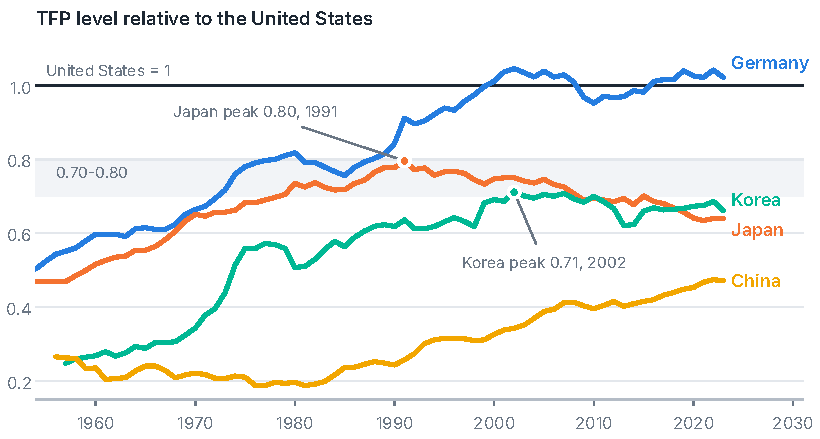
\includegraphics[width=0.9\textwidth,height=0.62\textheight,keepaspectratio]{figures/fig2_tfp.pdf}
\caption*{Figure L.1. Total factor productivity relative to the United
States (PWT 11.0, ctfp), 1954-2023.}
\end{figure}

The two completed East Asian cases stalled between 0.70 and 0.80 of the
American level of total factor productivity (TFP) after the escalation
phase. TFP is output per unit of combined inputs; the figure uses the
Penn World Table (PWT) measure at current purchasing power parities
(ctfp). Japan peaked at 0.80 of the American level in 1991 and fell back
to 0.64 by 2023. Korea peaked at 0.71 in 2002 and has stayed between
0.62 and 0.70 since 2010. Germany has been at or above the American
level for most years since 2000. Part of its rise in the early 1990s
reflects unification. China reached 0.47 in 2023, after a pause at about
0.40 to 0.42 between 2007 and 2015 (\texttt{data/\allowbreak{}ds3\_\allowbreak{}tfp.csv}).

This pattern is descriptive. Domestic explanations remain strong
(Acemoglu, Aghion and Zilibotti 2006; Eichengreen, Park and Shin 2012).
In a sample of this size, regression to the mean would produce the same
observations (Pritchett and Summers 2014). China's pause began at a much
lower level. It therefore appears to reflect domestic misallocation, and
an approach to the frontier seems an unlikely cause.

\hypertarget{references-for-the-appendix}{%
\section*{References for the
appendix}\label{references-for-the-appendix}}
\addcontentsline{toc}{section}{References for the appendix}

Acemoglu, D., Aghion, P. and Zilibotti, F. (2006) `Distance to frontier,
selection, and economic growth', \emph{Journal of the European Economic
Association}, 4(1), pp.~37-74.

Adams, W. (1979) `Import restraints and industrial performance: the
dilemma of protectionism', \emph{Michigan Yearbook of International
Legal Studies} (now \emph{Michigan Journal of International Law}), 1(1),
pp.~34-52.

Bailey, M. A., Strezhnev, A. and Voeten, E. (2017) `Estimating dynamic
state preferences from United Nations voting data', \emph{Journal of
Conflict Resolution}, 61(2), pp.~430-456.

Ballinger, R. A. (1978) \emph{A History of Sugar Marketing Through
1974}. Agricultural Economic Report No.~382. Washington, DC: US
Department of Agriculture, Economics, Statistics, and Cooperatives
Service, March.

Berry, S., Levinsohn, J. and Pakes, A. (1999) `Voluntary export
restraints on automobiles: evaluating a trade policy', \emph{American
Economic Review}, 89(3), pp.~400-431.

Bolt, J. and van Zanden, J. L. (2024) `Maddison-style estimates of the
evolution of the world economy: a new 2023 update', \emph{Journal of
Economic Surveys}, 39(2), pp.~631-671. Data: Maddison Project Database
2023, DataverseNL, doi:10.34894/INZBF2.

Bown, C. P. (2016) \emph{Temporary Trade Barriers Database}. World Bank
Data Catalog, dataset 0039583.

Bown, C. P. and Crowley, M. A. (2013a) `Import protection, business
cycles, and exchange rates: evidence from the Great Recession',
\emph{Journal of International Economics}, 90(1), pp.~50-64.

Bush, G. H. W. (1990) `Statement on United States action against foreign
trade barriers', 26 May 1989, in \emph{Public Papers of the Presidents
of the United States: George Bush, 1989}, Book I. Washington, DC: Office
of the Federal Register, pp.~607-608.

Chamberlain, J. (1903) \emph{Imperial Union and Tariff Reform: Speeches
Delivered from May 15 to Nov.~4, 1903}. London: Grant Richards.

Conlon, M. (2010) \emph{The History of U.S. Cotton in Japan}. GAIN
Report JA0503. Tokyo: USDA Foreign Agricultural Service, Agricultural
Trade Office Tokyo, 12 April. Available at:
https://www.usdajapan.org/wpusda/wp-content/uploads/2016/04/The-History-of-U.S.-Cotton-in-Japan-\_Tokyo-ATO\_Japan\_4-12-2010.pdf
(Accessed: 25 November 2026).

Crafts, N. F. R. (1989) `Revealed comparative advantage in
manufacturing, 1899-1950', \emph{Journal of European Economic History},
18(1), pp.~127-137.

Defense Science Board (1987) \emph{Report of the Defense Science Board
Task Force on Defense Semiconductor Dependency}. Washington, DC: Office
of the Under Secretary of Defense for Acquisition, February. DTIC
ADA178284.

Dinopoulos, E. and Kreinin, M. E. (1991) `The U.S. VER on machine tools:
causes and effects', in R. E. Baldwin (ed.) \emph{Empirical Studies of
Commercial Policy}. Chicago: University of Chicago Press, pp.~113-134.

Eichengreen, B., Park, D. and Shin, K. (2012) `When fast-growing
economies slow down: international evidence and implications for China',
\emph{Asian Economic Papers}, 11(1), pp.~42-87.

Ericsson (2013) \emph{Annual Report 2012}. Stockholm:
Telefonaktiebolaget LM Ericsson.

European Commission (2013) `EU imposes provisional anti-dumping duties
on Chinese solar panels', MEMO/13/497, 4 June. Available at:
https://ec.europa.eu/commission/presscorner/detail/en/MEMO\_13\_497
(Accessed: 25 November 2026).

European Commission (2024) `EU imposes duties on unfairly subsidised
electric vehicles from China while discussions on price undertakings
continue', IP/24/5589, 29 October. Available at:
https://ec.europa.eu/commission/presscorner/detail/en/ip\_24\_5589
(Accessed: 25 November 2026).

European Commission and High Representative (2019) \emph{EU-China -- A
Strategic Outlook}, JOIN(2019) 5 final, Strasbourg, 12 March.

Flamm, K. (1996) \emph{Mismanaged Trade? Strategic Policy and the
Semiconductor Industry}. Washington, DC: Brookings Institution Press.

Fouquin, M. and Hugot, J. (2016) \emph{Two Centuries of Bilateral Trade
and Gravity Data: 1827-2014}. CEPII Working Paper No.~2016-14. Paris:
CEPII.

FRUS (1987) \emph{Foreign Relations of the United States, 1955-1957,
Vol. IX: Foreign Economic Policy; Foreign Information Program}.
Washington, DC: Government Printing Office. Doc. 99: report by Herbert
N. Blackman, Department of Commerce, 12 July 1957. Available at:
https://history.state.gov/historicaldocuments/frus1955-57v09/d99
(Accessed: 25 November 2026).

Gao, Z. and Tisdell, C. (2004) `Television production: its changing
global location, the product cycle and China', Working Papers on
Economic Theory, Applications and Issues No.~26. Brisbane: The
University of Queensland, January.

House of Commons (1888) \emph{Return (in continuation of Parliamentary
Paper, No.~312, of Session 1887), bringing the Tables therein up to
Date, together with such later Information as can be given on the
Employment of Labour in the various Sugar Industries of the United
Kingdom}. House of Commons Papers 1888, No.~353. London: Henry Hansard
and Son.

Huawei (2013) `Huawei announces 2012 financial results', 21 January.
Available at: https://www.huawei.com/au/news/au/2013/hw-201987
(Accessed: 25 November 2026).

Hufbauer, G. C. and Vieiro, M. (2012) `US anti-dumping duties on Chinese
solar cells: a costly step', \emph{Realtime Economic Issues Watch},
Peterson Institute for International Economics, 25 May. Available at:
https://www.piie.com/blogs/realtime-economic-issues-watch/us-anti-dumping-duties-chinese-solar-cells-costly-step
(Accessed: 25 November 2026).

Irwin, D. A. (1996) `Trade policies and the semiconductor industry', in
A. O. Krueger (ed.) \emph{The Political Economy of American Trade
Policy}. Chicago: University of Chicago Press, pp.~11-72.

Kane, M. (2024) `Top all-electric car OEMs by sales in Q4 and 2023:
Tesla vs.~BYD', \emph{InsideEVs}, 16 January. Available at:
https://insideevs.com/news/704678/top-electric-car-oems-sales-2023q4-tesla-byd/
(Accessed: 25 November 2026).

Kentikelenis, A. E., Stubbs, T. H. and King, L. P. (2016) `IMF
conditionality and development policy space, 1985-2014', \emph{Review of
International Political Economy}, 23(4), pp.~543-582.

Kocka, J. (1971) `Family and bureaucracy in German industrial
management, 1850-1914: Siemens in comparative perspective',
\emph{Business History Review}, 45(2), pp.~133-156. doi:10.2307/3113099.

Kuziemko, I. and Werker, E. (2006) `How much is a seat on the Security
Council worth? Foreign aid and bribery at the United Nations',
\emph{Journal of Political Economy}, 114(5), pp.~905-930.

League of Nations (1945) \emph{Industrialization and Foreign Trade}.
Geneva: League of Nations.

Leeds, B. A., Ritter, J. M., Mitchell, S. M. and Long, A. G. (2002)
`Alliance Treaty Obligations and Provisions, 1815-1944',
\emph{International Interactions}, 28(3), pp.~237-260.

Moore, M. O. (1996) `Steel protection in the 1980s: the waning influence
of big steel?', in A. O. Krueger (ed.) \emph{The Political Economy of
American Trade Policy}. Chicago: University of Chicago Press,
pp.~73-132.

Murmann, J. P. and Homburg, E. (2001) `Comparing evolutionary dynamics
across different national settings: the case of the synthetic dye
industry, 1857-1914', \emph{Journal of Evolutionary Economics}, 11(2),
pp.~177-205.

NBER (n.d.) \emph{NBER Macrohistory Database}, series 01183B (United
Kingdom, steel ingots) and 01216 (Germany and Luxembourg, steel).
Cambridge, MA: National Bureau of Economic Research. Available at:
https://www.nber.org/research/data/nber-macrohistory-i-production-commodities
(Accessed: 25 November 2026).

Ohashi, H. (2005) `Learning by doing, export subsidies, and industry
growth: Japanese steel in the 1950s and 1960s', \emph{Journal of
International Economics}, 66(2), pp.~297-323.

Pritchett, L. and Summers, L. H. (2014) \emph{Asiaphoria Meets
Regression to the Mean}. NBER Working Paper 20573.

Reagan, R. (1989) `Statement on tariff increases on Japanese
semiconductor products', 17 April 1987, in \emph{Public Papers of the
Presidents of the United States: Ronald Reagan, 1987}, Book I.
Washington, DC: Office of the Federal Register, pp.~382-383.

Robson, R. (1957) \emph{The Cotton Industry in Britain}. London:
Macmillan.

Rogin, J. (2012) `NSA chief: cybercrime constitutes the ``greatest
transfer of wealth in history''\,', \emph{Foreign Policy} (The Cable), 9
July. Available at:
https://foreignpolicy.com/2012/07/09/nsa-chief-cybercrime-constitutes-the-greatest-transfer-of-wealth-in-history/
(Accessed: 25 November 2026).

Samsung Semiconductor (n.d.) `History'. Available at:
https://semiconductor.samsung.com/about-us/history/ (Accessed: 25
November 2026).

Sandberg, L. G. (1974) \emph{Lancashire in Decline: A Study in
Entrepreneurship, Technology, and International Trade}. Columbus: Ohio
State University Press.

Schneider, F., Jr.~(1926) `Sugar', \emph{Foreign Affairs}, 4(2),
pp.~311-320. doi:10.2307/20028448.

Semiconductor History Museum of Japan (n.d.) `80s trends in the
semiconductor industry'. Available at:
https://www.shmj.or.jp/english/trends/trd80s.html (Accessed: 25 November
2026).

Sobel, R. (1984) \emph{Car Wars: The Untold Story}. New York: Dutton.

Stubbs, T. H., Kentikelenis, A. E. and King, L. P. (2016) `Catalyzing
aid? The IMF and donor behavior in aid allocation', \emph{World
Development}, 78, pp.~511-528.

Stubbs, T., Reinsberg, B., Kentikelenis, A. and King, L. (2020) `How to
evaluate the effects of IMF conditionality', \emph{Review of
International Organizations}, 15(1), pp.~29-73.

Sugihara, K. (1999) `International circumstances surrounding the postwar
Japanese cotton textile industry', Discussion Papers in Economics and
Business 99-06. Osaka: Graduate School of Economics, Osaka University,
March.

Tan, J. (2018) `Huawei now world's largest telecom equipment-maker',
\emph{Caixin Global}, 19 March. Available at:
https://www.caixinglobal.com/2018-03-19/huawei-now-worlds-largest-telecom-equipment-maker-101223256.html
(Accessed: 25 November 2026).

TechInsights (2023) `TechInsights finds SMIC 7nm (N+2) in Huawei Mate 60
Pro', 4 September. Available at:
https://www.techinsights.com/blog/techinsights-finds-smic-7nm-n2-huawei-mate-60-pro
(Accessed: 25 November 2026).

Tesla (2024) `Tesla vehicle production \& deliveries and date for
financial results \& webcast for fourth quarter 2023', 2 January.
Austin, TX: Tesla, Inc.

The Japan Times (2002) `Japan back to No.~1 in shipbuilding', 18
February. Available at:
https://www.japantimes.co.jp/news/2002/02/18/business/japan-back-to-no-1-in-shipbuilding/
(Accessed: 25 November 2026).

Time (1957) `Foreign trade: textile compromise', \emph{Time}, 28
January.

Toyota Motor Corporation (2012) `75 Years of Toyota. Part 3, Chapter 1,
Section 1: Voluntary restraints imposed on exports to U.S.; Item 3: U.S.
sales structure strengthened amid voluntary restraints'. Available at:
https://www.toyota-global.com/company/history\_of\_toyota/75years/text/leaping\_forward\_as\_a\_global\_corporation/chapter1/section1/item3.html
(Accessed: 25 November 2026).

Tyszynski, H. (1951) `World trade in manufactured commodities,
1899-1950', \emph{The Manchester School}, 19(3), pp.~272-304.

Urata, S. (2020) `US-Japan trade frictions: the past, the present, and
implications for the US-China trade war', \emph{Asian Economic Policy
Review}, 15(1), pp.~141-159. doi:10.1111/aepr.12279.

US Department of Commerce (2012a) `Crystalline silicon photovoltaic
cells, whether or not assembled into modules, from the People's Republic
of China: final affirmative countervailing duty determination and final
affirmative critical circumstances determination', \emph{Federal
Register}, 77, 17 October, pp.~63788-63791.

US Department of Commerce (2012b) `Crystalline silicon photovoltaic
cells, whether or not assembled into modules, from the People's Republic
of China: final determination of sales at less than fair value, and
affirmative final determination of critical circumstances, in part',
\emph{Federal Register}, 77, 17 October, pp.~63791-63798.

US Senate, Committee on Energy and Natural Resources (2012) \emph{Clean
Energy Race: The United States and China}. Hearing, 112th Congress, 2nd
session, 14 June 2012, S. Hrg. 112-623. Washington, DC: U.S. Government
Printing Office.

US Tariff Commission (1971) \emph{Television Receiving Sets from Japan:
Determination of Injury in Investigation No.~AA1921-66 under the
Antidumping Act, 1921, as Amended}. TC Publication 367. Washington, DC,
March.

USCC (2023) \emph{2023 Report to Congress of the U.S.-China Economic and
Security Review Commission}. Washington, DC: U.S.-China Economic and
Security Review Commission, 30 November.

USITC (1978) \emph{The History and Current Status of the Multifiber
Arrangement}. USITC Publication 850. Washington, DC: U.S. International
Trade Commission, January.

USITC (1983) \emph{Foreign Industrial Targeting and Its Effects on U.S.
Industries, Phase I: Japan}. Investigation No.~332-162, USITC
Publication 1437. Washington, DC: U.S. International Trade Commission,
October.

USITC (1985) \emph{The Internationalization of the Automobile Industry
and Its Effects on the U.S. Automobile Industry}. Investigation
No.~332-188, USITC Publication 1712. Washington, DC: U.S. International
Trade Commission, June.

USITC (2003) \emph{DRAMs and DRAM Modules from Korea}. Investigation
No.~701-TA-431 (Final), USITC Publication 3616. Washington, DC: U.S.
International Trade Commission, August.

USITC (2020) \emph{Crystalline Silicon Photovoltaic Cells, Whether or
Not Partially or Fully Assembled Into Other Products: Monitoring
Developments in the Domestic Industry}. Investigation No.~TA-201-075
(Monitoring), USITC Publication 5021. Washington, DC: U.S. International
Trade Commission, February.

USTR (2018a) `USTR issues tariffs on Chinese products in response to
unfair trade practices', 15 June. Available at:
https://ustr.gov/about-us/policy-offices/press-office/press-releases/2018/june/ustr-issues-tariffs-chinese-products
(Accessed: 25 November 2026).

USTR (2018b) `Notice of action and request for public comment concerning
proposed determination of action pursuant to Section 301: China's acts,
policies, and practices related to technology transfer, intellectual
property, and innovation', \emph{Federal Register}, 83, 20 June,
pp.~28710-28756.

USTR (2019) `United States and China reach Phase One trade agreement',
13 December. Available at:
https://ustr.gov/about-us/policy-offices/press-office/press-releases/2019/december/united-states-and-china-reach
(Accessed: 25 November 2026).

USTR (2024a) \emph{Four-Year Review of Actions Taken in the Section 301
Investigation: China's Acts, Policies, and Practices Related to
Technology Transfer, Intellectual Property, and Innovation}. Washington,
DC: Office of the United States Trade Representative, 14 May.

USTR (2024b) `U.S. Trade Representative Katherine Tai to take further
action on China tariffs after releasing statutory four-year review', 14
May. Available at:
https://ustr.gov/about-us/policy-offices/press-office/press-releases/2024/may/us-trade-representative-katherine-tai-take-further-action-china-tariffs-after-releasing-statutory
(Accessed: 25 November 2026).

USTR (2024c) `Notice of modification: China's acts, policies and
practices related to technology transfer, intellectual property and
innovation', \emph{Federal Register}, 89, 18 September, pp.~76581-76614.

Wade, R. H. (2003) `What strategies are viable for developing countries
today? The World Trade Organization and the shrinking of ``development
space''\,', \emph{Review of International Political Economy}, 10(4),
pp.~621-644.

White House (1987) `Statement by Deputy Press Secretary for Foreign
Affairs Djerejian on the South Korea-United States trade policy', 21
July 1986, in \emph{Public Papers of the Presidents of the United
States: Ronald Reagan, 1986}, Book II. Washington, DC: Office of the
Federal Register, pp.~978-979.

White House (2022) `Remarks by National Security Advisor Jake Sullivan
at the Special Competitive Studies Project Global Emerging Technologies
Summit', 16 September. Available at:
https://bidenwhitehouse.archives.gov/briefing-room/speeches-remarks/2022/09/16/remarks-by-national-security-advisor-jake-sullivan-at-the-special-competitive-studies-project-global-emerging-technologies-summit/
(Accessed: 25 November 2026).

Williams, E. E. (1896) \emph{Made in Germany}. London: William
Heinemann.

World Bank (2026) \emph{World Development Indicators}, series
NV.IND.MANF.CD (manufacturing, value added, current US dollars).
Available at: https://data.worldbank.org (Accessed: 25 November 2026).

WTO (1995) `Article XXXV: non-application of the Agreement', in
\emph{Analytical Index of the GATT}. Geneva: World Trade Organization,
pp.~1031-1038 (citing GATT document L/405, September 1955).

WTO (2018) \emph{Korea -- Measures Affecting Trade in Commercial
Vessels}, DS571, request for consultations by Japan, 6 November.

WTO (2020) \emph{Korea -- Measures Affecting Trade in Commercial Vessels
(Second Complaint)}, DS594, request for consultations by Japan, 31
January.

Primary legal and parliamentary sources are cited in the tables by their
official reference and are not repeated here: the Federal Register by
volume and page (FR), Presidential proclamations by number, US public
laws by number and Statutes at Large page, British statutes by regnal
year and chapter, the Official Journal of the European Union by series,
number and date, Hansard by house and date (Historic Hansard), the
London Gazette by issue and page, and GATT documents by symbol.
